\begin{greek}

\chapter{Παράλληλη συλλογή σκουπιδιών}\label{ch:par}
Μέχρι τώρα έχουμε υποθέσει πώς, ενώ ο τροποποιητής μπορεί να
είναι πολυνηματικός, ο συλλέκτης είναι μονονηματικός. Η υπόθεση
αυτή οδηγεί σε φτωχή εκμετάλλευση των πόρων ενός σύγχρονου
πολυπύρηνου μηχανήματος. Στο παρόν κεφάλαιο εξετάζουμε πώς
μπορεί να παραλληλοποιηθεί ο συλλέκτης, υποθέτοντας ακόμα πώς
κανένα από τα νήματα του τροποποιητή δεν εκτελείται ενώ
πραγματοποιείται συλλογή σκουπιδιών και πώς αυτή ολοκληρώνεται
πριν αυτά συνεχίσουν την εκτέλεσή τους. Ένας προφανής τρόπος
προκειμένου να μειωθεί ο χρόνος παύσης των νημάτων τροποποιητών
είναι οι πυρήνες να συνεργαστούν κατά τη συλλογή σκουπιδιών
(και ενώ τα νήματα του τροποποιητή είναι σταματημένα). Η 
\textbf{παράλληλη συλλογή σκουπιδιών} είναι το αντικείμενο
αυτού του κεφαλαίου. Πιο συγκεκριμένα θα εξετάσουμε πώς μπορούν
να παραλληλοποιηθούν οι τέσσερις βασικές διαδικασίες της συλλογής
με εξιχνίαση: σήμανση, εκκαθάριση, αντιγραφή και συμπύκνωση.

\begin{figure}[H]
  \centering
  \begin{subfigure}{1.0\textwidth}
    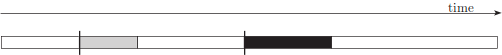
\includegraphics{figures/par_1a}
    \caption
      {Συλλογή με παύση του κόσμου, μονονηματικός τροποποιητής, 
       μονονηματικός συλλέκτης.}
  \end{subfigure}

  \begin{subfigure}[b]{1.0\textwidth}
    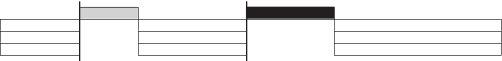
\includegraphics{figures/par_1b}
    \caption
      {Συλλογή με παύση του κόσμου, πολυνηματικός τροποποιητής,
       μονονηματικός συλλέκτης.}
  \end{subfigure}
  
  \begin{subfigure}[b]{1.0\textwidth}
    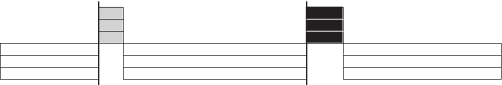
\includegraphics{figures/par_1c}
    \caption
      {Συλλογή με παύση του κόσμου, πολυνηματικός τροποποιητής,
       πολυνηματικός συλλέκτης.}
  \end{subfigure}
  
  \caption
    [Συλλογή σκουπιδιών με παύση του κόσμου: κάθε μπάρα αναπαριστά
     την εκτέλεση σε έναν επεξεργαστή.]
    {Συλλογή σκουπιδιών με παύση του κόσμου: κάθε μπάρα αναπαριστά
     την εκτέλεση σε έναν επεξεργαστή. Οι χρωματισμένες περιοχές
     αναπαριστούν διαφορετικούς κύκλους συλλογής σκουπιδιών.}
  \label{fig:par_1}
\end{figure}

\section{Υπάρχει επαρκής δουλειά προς παραλληλοποίηση;}
Όπως και κατά την παραλληλοποίηση του αλγορίθμου οποιουδήποτε
προβλήματος, η πρώτη απαίτηση αφορά στην εξασφάλιση του ότι
το φορτίο εργασίας είναι αρκετά μεγάλο ώστε η παραλληλοποίηση
να αξίζει τον κόπο. Αναπόφευκτα, η παράλληλη συλλογή σκουπιδιών
απαιτεί κάποια μορφή συγχρονισμού των νημάτων συλλεκτών με το
συγχρονισμό αυτό να κοστίζει. Ο συγχρονισμός αυτός μπορεί να
επιτευχθεί με τη χρήση είτε κλειδωμάτων είτε ατομικών πρωταρχικών
λειτουργιών υλικού όπως για παράδειγμα της \textproc{CompareAndSwap}
και την προσεκτική σχεδίαση βοηθητικών δομών δεδομένων. Προκύπτει
λοιπόν το ερώτημα αν το φορτίο εργασίας της συλλογής σκουπιδιών
επαρκεί ώστε το κέρδος από την παραλληλοποίηση να υπερκερνά το
κόστος του συγχρονισμού.

Aς υποθέσουμε για παράδειγμα, πώς ένας συλλέκτης με σήμανση
και εκκαθάριση θα πρέπει να σημάνει μία απλή συνδεδεμένη λίστα:
σε κάθε βήμα, η στοίβα σήμανσης θα περιέχει μόνο ένα αντικείμενο,
τον επόμενο κόμβο προς εξέταση. Στην περίπτωση αυτή, μόνο ένα από
τα νήματα συλλέκτες θα δουλεύει, ενώ τα υπόλοιπα θα είναι αδρανή,
περιμένοντας για δουλειά. Ο Siebert \cite{DBLP:conf/iwmm/Siebert08}
αποδεικνύει πώς ο αριθμός φορών $n$ που ένας επεξεργαστής μένει
αδρανής κατά τη διάρκεια μιας παράλληλης σήμανσης σε ένα σύστημα
με $p$ επεξεργαστές φράσσεται από το μέγιστο βάθος των προσβάσιμων
αντικειμένων $o$:

\begin{equation}
  n \leq (p-1) \cdot \max_{o \in reachable}{depth(o)}
  \label{eq:par_1}
\end{equation}

Η ανίσωση αυτή πάντως βασίζεται στην όχι ρεαλιστική υπόθεση
πώς όλα τα βήματα σήμανσης διαρκούν το ίδιο, κάτι που δεν ισχύει
καθώς οι χρόνοι διαφέρουν ανάλογα με το μέγεθος του αντικειμένου.
Στις περισσότερες γλώσσες προγραμματισμού πάντως η μεγάλη πλειοψηφία
των αντικειμένων είναι μικρά (περιέχουν λίγους δείκτες).

Μελέτες πάντως έχουν δείξει πώς οι τυπικές εφαρμογές περιλαμβάνουν
μια ευρεία ποικιλία από πλούσιες σε δείκτες δομές δεδομένων.
Για παράδειγμα, η εξιχνίαση μιας δενδροειδούς δομής δεδομένων
θα παράγει περισσότερες μονάδες εργασίας από όσες θα καταναλώνει
μέχρις ότου η εξερεύνηση φθάσει στα φύλλα.

\section{Εξισορρόπηση φορτίου}
Μια άλλη απαίτηση από την παράλληλη συλλογή σκουπιδιών είναι
το φορτίο της συλλογής να κατανεμηθεί με τέτοιο τρόπο ώστε να
ελαχιστοποιηθεί η ανάγκη για συντονισμό και όλοι οι επεξεργαστές
να είναι απασχολημένοι ταυτόχρονα. Ο Endo κ.ά \cite{DBLP:conf/sc/EndoTY97}
διαπιστώνουν πώς χωρίς κάποιο μηχανισμό για \textbf{εξισορρόπηση
φορτίου}, μια απλοϊκή παραλληλοποίηση μπορεί να οδηγήσει σε
πολύ μικρή επιτάχυνση σε πολυεπεξεργαστικά συστήματα.

Δυστυχώς, ο στόχος της ομοιόμορφης κατανομής υπολογιστικού φορτίου
και της ελαχιστοποίησης του απαιτούμενου συντονισμού αλληλοσυγκρούονται.
Ο στατικός διαμοιρασμός του υπολογιστικού φόρτου δεν είναι
πάντα ο καλύτερος. Για παράδειγμα, έστω ένας παράλληλος συλλέκτης
με σήμανση και συμπύκνωση σε σύστημα N επεξεργαστών. Αν ο σωρός
διαιρεθεί σε $N$ τμήματα, και ο κάθε επεξεργαστής αναλάβει την
επιδιόρθωση των δεικτών στο δικό του τμήμα, τότε, αν ο αριθμός
των αντικειμένων και των δεικτών που αυτά περιέχουν ποικίλλει
πολύ από τμήμα σε τμήμα, κάποιοι επεξεργαστές θα δουλεύουν
περισσότερο από άλλους. Εξίσου σημαντική με την εξισορρόπηση
του υπολογιστικού φορτίου ανάμεσα στους επεξεργαστές είναι
και η εξισορρόπηση άλλων πόρων. Σε μία παράλληλη υλοποίηση
του αλγόριθμου αντιγραφής του Baker \cite{DBLP:journals/cacm/Baker78},
ο Halstead \cite{DBLP:conf/lfp/Halstead84, DBLP:journals/toplas/Halstead85}
ανέθεσε σε κάθε επεξεργαστή το δικό του χώρο-προς και χώρο-από.
Δυστυχώς, αυτός ο στατικός διαμοιρασμός συχνά οδηγούσε σε μία
κατάσταση όπου ένας επεξεργαστής εξαντλούσε το δικό του χώρο-από
και ενώ υπήρχε χώρος στους χώρους-από των υπολοίπων επεξεργαστών.

Ένας \textbf{δυναμικός διαμοιρασμός} είναι περισσότερο κατάλληλος
προκειμένου η δουλειά να μοιραστεί σχεδόν ομοιόμορφα. Ας θεωρήσουμε
για παράδειγμα ένα συλλέκτη με σήμανση και εκκαθάριση: αφού έχει
ολοκληρωθεί η σήμανση των ζωντανών αντικειμένων, ο σωρός διαχωρίζεται
σε $Ν$ τμήματα, τα οποία έχουν παρόμοιο πλήθος ζωντανών αντικειμένων
και δεικτών. Στη συνέχεια, οι επεξεργαστές συμπυκνώνουν παράλληλα
ο καθένας το δικό του τμήμα του σωρού. Αυτή είναι ακριβώς η
προσέγγιση των Flood κ.ά \cite{DBLP:conf/jvm/FloodDSZ01}.

Συχνά η εξαρχής εκτίμηση εργασίας για την καλύτερη διαίρεσή της
δεν είναι εφικτή. Σε αυτήν την περίπτωση η συνηθισμένη λύση
είναι να \textbf{υπερ-διαμερίζεται} η συνολική εργασία ούτως
ώστε να υπάρχουν περισσότερα τμήματα εργασίας από ότι επεξεργαστές
ή νήματα και οι επεξεργαστές (ή τα νήματα) να τίθενται σε
ανταγωνισμό για την απόκτηση τους. Βασικό πλεονέκτημα της τεχνικής
αυτής αποτελεί το γεγονός πώς είναι ανθεκτική σε αλλαγές του
διαθέσιμου πλήθους επεξεργαστών στο συλλέκτη (π.χ. λόγω της
επιβάρυνσης από άλλες διεργασίες που εκτελούνται παράλληλα), καθώς
οι μικρότερες μονάδες εργασίες ανταλλάσσονται πιο εύκολα.

Απλοποιούμε τους αλγορίθμους που θα παρουσιάσουμε αργότερα εστιάζοντας
την προσοχή μας στις τρεις βασικές υπο-εργασίες της απόκτησης,
εκτέλεσης και δημιουργίας δουλειάς συλλογής. Θεωρούμε λοιπόν πώς,
στις περισσότερες περιπτώσεις, κάθε νήμα του συλλέκτη εκτελεί
τον ακόλουθο βρόχο:

\begin{algorithm}
  \caption{Παράλληλη συλλογή σκουπιδιών}
  \label{alg:par_1}
  \begin{algorithmic}[1]
    \Procedure{run}{\null}
      \While{\textbf{not} \Call{terminated}{\null}}
        \State \Call{acquireWork}{\null}
        \State \Call{performWork}{\null}
        \State \Call{generateWork}{\null}
      \EndWhile
    \EndProcedure
  \end{algorithmic}
\end{algorithm}

\section{Συγχρονισμός}
Εκ πρώτης όψεως ίσως φαίνεται πώς η βέλτιστη στρατηγική
εξισορρόπησης του φορτίου εργασίας είναι η διαίρεση του στις
ελάχιστες δυνατές υποεργασίες, όπως για παράδειγμα η σήμανση
ή η αντιγραφή ενός μόνο αντικειμένου. Παρότι η λύση αυτή πετυχαίνει
τέλειο διαμοιρασμό εργασίας ανάμεσα στους επεξεργαστές, το
κόστος που επιβάλλει ο συντονισμός των τελευταίων την καθιστά
απαγορευτική. Ο συγχρονισμός απαιτείται τόσο για την εξασφάλιση
της ορθότητας όσο και για την αποφυγή της επανάληψης, ή
τουλάχιστον ελαχιστοποίησης της εκτέλεσης ορισμένων μονάδων
εργασίας περισσότερες από μια φορές.

Η επίτευξη συγχρονισμού μεταξύ των νημάτων συλλεκτών κοστίζει
σε χρόνο και σε χώρο. Οι μηχανισμοί που εξασφαλίζουν αποκλειστικότητα
πρόσβασης χρησιμοποιούν μεταξύ άλλων κλειδώματα ή δομές
δεδομένων χωρίς αναμονή. Οι καλώς σχεδιασμένοι αλγόριθμοι
ελαχιστοποιούν τις περιπτώσεις όπου απαιτούνται ενέργειες
συγχρονισμού, παρέχοντας για παράδειγμα σε κάθε νήμα ιδιωτικές
τοπικές δομές δεδομένων. Σε μερικές περιπτώσεις πάντως η
μη αποκλειστική πρόσβαση δεν είναι απαραίτητη για την εξασφάλιση
της ορθότητας και έτσι κάποιες ενέργειες συγχρονισμού μπορούν
να παραληφθούν.

Οι μοντέρνες υλοποιήσεις παράλληλης συλλογής σκουπιδιών συνήθως
θέτουν να νήματα εργασίας σε ανταγωνισμό για την απόκτηση
μονάδων εργασίας, τις οποίες στη συνέχεια εκτελούν χωρίς περαιτέρω
συγχρονισμό. Οι μονάδες εργασίας οργανώνονται είτε ως τοπικές
στοίβες σήμανσης, είτε ως ξεχωριστές περιοχές του σωρού προς
σάρωση είτε ως καθολικές δεξαμενές. Οι βοηθητικές δομές δεδομένων
για την οργάνωση των μονάδων εργασίας επιβάλλουν ένα κόστος σε
χώρο για την αποθήκευση των μεταδεδομένων τους, το οποίο όμως
τείνει να είναι μικρό.

\section{Ταξινόμηση}
Στο υπόλοιπο του κεφαλαίου παρουσιάζουμε ειδικές λύσεις στο
πρόβλημα της παραλληλοποίησης της σήμανσης, της εκκαθάρισης,
της αντιγραφής και της συμπύκνωσης. Σε όλες τις περιπτώσεις
ενδιαφερόμαστε στο πώς οι αλγόριθμοι αποκτούν, εκτελούν και
παράγουν εργασίες. Η σχεδίαση και η υλοποίηση αυτών των τριών
δραστηριοτήτων καθορίζει τον απαιτούμενο συγχρονισμό, τη
διακριτότητα των φορτίων εργασίας των νημάτων καθώς επίσης
και πώς αυτά τα φορτία διαμοιράζονται ομοιόμορφα μεταξύ
επεξεργαστών.

Οι αλγόριθμοι παράλληλης συλλογής σκουπιδιών μπορούν να
κατηγοριοποιηθούν με βάση το αν στο επίκεντρο της σχεδίασης
είναι ο επεξεργαστής ή η μνήμη. Οι αλγόριθμοι της πρώτης
κατηγορίας τείνουν να επιτρέπουν στα νήματα να αποκτούν κβάντα
εργασίας μεταβλητού μεγέθους, συνήθως κλέβοντας εργασία
από άλλα νήματα. Λίγη έως και καθόλου σημασία δίνεται στην
τοποθεσία των αντικειμένων στη μνήμη, παρότι η τοπικότητα
επηρεάζει την επίδοση ακόμη και σε μονοπύρηνες αρχιτεκτονικές.
Οι αλγόριθμοι της δεύτερης κατηγορίας από την άλλη πλευρά
λαμβάνουν περισσότερο υπόψην τους τη θέση των αντικειμένων
στη μνήμη. Συνήθως λειτουργούν σε συνεχόμενα μπλοκ μνήμης
σωρού και αποκτούν/κατεθέτουν εργασία από/προς μοιραζόμενες
δεξαμενές.

Τέλος, εξετάζουμε τον τερματισμό της παράλληλης συλλογής
σκουπιδιών. Συνήθως, απλώς η εξέταση του κατά πόσο μια δεξαμενή
εργασίας είναι κενή δεν επαρκεί, καθώς ένα ενεργό νήμα μπορεί
να ετοιμάζεται να καταθέσει καινούριες μονάδες εργασίας σε αυτή.

\section{Παράλληλη Σήμανση}
Η φάση της σήμανσης, σε αντίθεση με τις φάσεις της εκκαθάρισης
και της συμπύκνωσης δεν είναι εγγενώς παραλληλοποιήσιμη.

\subsection{Κλοπή εργασιών}
Οι Endo κ.ά \cite{DBLP:conf/sc/EndoTY97}, Flood κ.ά \cite{DBLP:conf/jvm/FloodDSZ01}
καθώς και ο Siebert \cite{DBLP:conf/iwmm/Siebert10} χρησιμοποιούν 
\textbf{κλοπή εργασίας (work stealing)} για την εξισορρόπηση
του υπολογιστικού φόρτου. Οποτεδήποτε ένα νήμα ξεμένει από
δουλειά σήμανσης, κλέβει δουλειά που ανήκει σε ένα άλλο νήμα.
Σε μία παράλληλη υλοποίηση του συντηρητικού συλλέκτη των Boehm
και Weiser \cite{DBLP:journals/spe/BoehmW88}, ο Endo κ.ά παρέχουν
σε κάθε νήμα σήμανσης την δική του τοπική στοίβα σήμανσης καθώς
επίσης και μία \textbf{κλεπτόμενη ουρά εργασιών}. Περιοδικά,
κάθε νήμα ελέγχει την κλεπτόμενη ουρά εργασιών του και αν αυτή
είναι άδεια, μεταφέρει όλη την ιδιωτική στοίβα σήμανσης του (εκτός
των τοπικών ριζών) στην ουρά. Ένα αδρανές νήμα αποκτά έργο σήμανσης
ελέγχοντας αρχικά την δική του κλεπτόμενη ουρά και στη συνέχεια
τις κλεπτόμενες ουρές των άλλων νημάτων. Όταν ένα νήμα βρει μια
μη κενή κλεπτόμενη ουρά, κλέβει τις μισές καταχωρίσεις αυτής
και τις μεταφέρει στην ιδιωτική του στοίβα σήμανσης. Καθώς πολλά
νήματα προσπαθούν να κλέψουν δουλειά ταυτόχρονα, οι κλεπτόμενες
ουρές εργασιών προστατεύονται με κλειδώματα. 

Κάθε παράλληλος συλλέκτης οφείλει να είναι ιδιαίτερα προσεκτικός
όσον αφορά την ενημέρωση bitmap σήμανσης και την επεξεργασία
μεγάλων πινάκων. Τα bits μιας λέξης σε ένα bitmap σήμανσης πρέπει
να ενημερώνονται ατομικά. Αντί να κλειδώνουν ολόκληρη τη λέξη
όταν ελέγχουν ένα bit, ο Endo κ.ά χρησιμοποιούν μια απλή φόρτωση
για τον έλεγχο του bit και μόνον αν αυτό έχει την τιμή 0, επιχειρούν
ατομικά να εγγράψουν την τιμή 1 σε αυτό, προσπαθώντας εκ νέου,
αν η εγγραφή αποτύχει. Αντίθετα, συλλέκτες σαν αυτόν του Flood
κ.ά \cite{DBLP:conf/jvm/FloodDSZ01}, οι οποίοι αποθηκεύουν το
bit σήμανσης στην επικεφαλίδα του αντικειμένου μπορούν να
πραγματοποιούν σημάνσεις χωρίς τη χρήση ατομικών λειτουργιών.

Η επεξεργασία μεγάλων πινάκων αποτελεί πηγή πολλών προβλημάτων.
Για παράδειγμα, οι Boehn και Weiser \cite{DBLP:journals/spe/BoehmW88}
επιχειρούν να αποτρέψουν την υπερχείλιση της στοίβας σήμανσης
ωθώντας μεγάλα αντικείμενα σε τμήματα των 128 λέξεων. Παρόμοια,
και προκειμένου να βελτιώσουν την εξισορρόπηση φορτίου, ο Endo
κ.ά διαιρούν ένα μεγάλο αντικείμενο σε κομμάτια των 512 λέξεων 
πριν το τελευταίο εισαχθεί σε κάποια στοίβα σήμανσης ή κλεπτόμενη 
ουρά.

Ο παράλληλος γενεαλογικός συλλέκτης των Flood κ.ά \cite{DBLP:conf/jvm/FloodDSZ01}
διαχειρίζεται τη νέα γενιά με αντιγραφή και την παλαιά με
σήμανση και συμπύκνωση. Σε αυτήν την ενότητα εξετάζουμε μόνο
την παράλληλη σήμανση. Ενώ o Endo κ.ά χρησιμοποιούν μία στοίβα
και μια ουρά ανά επεξεργαστή, ο Flood κ.ά χρησιμοποιούν μία
\textbf{διπλά τερματισμένη ουρά (deque)} ανά νήμα σήμανσης.
Ο αλγόριθμος τους για κλοπή εργασίας δε χρησιμοποιεί κλειδώματα,
επιτρέπει το διαμοιρασμό εργασίας σε επίπεδο αντικειμένων και
βασίζεται στην ιδέα των Dimpsey κ.ά \cite{DBLP:journals/ibmsj/DimpseyAK00}.

\begin{algorithm}
  \caption{Παράλληλη σήμανση-εκκαθάριση: παράλληλη σήμανση με κλοπή εργασίας (Endo κ.ά)}
  \label{alg:par1}
  \begin{algorithmic}[1]
    \State \textbf{shared} \; stealableWorkQueue[N] \Comment{one per thread}
    \State $me \gets myThreadId$
    \Statex
    \Procedure{acquireWork}{\null}
      \If{\textbf{not} \Call{isEmpty}{$myMarkStack$}}
        \State \Return{\null}
      \EndIf
      \State \Call{lock}{$stealableWorkQueue[me]$}
      \State $n \gets$ \Call{size}{$stealableWorkQueue[me]$}/2 \Comment{grab half of my stealable work queue}
      \State \Call{transfer}{$stealableWorkQueue[me]$, $n$, $myMarkStack$}
      \State \Call{unlock}{$stealableWorkQueue[me]$}
      \If{\Call{isEmpty}{$myMarkStack$}}
        \ForAll{$j \; \textbf{in} \; Threads$}
          \If{\textbf{not} \Call{locked}{$stealableWorkQueue[j]$}}
            \If{\Call{lock}{$stealableWorkQueue[j]$}}
              \State $n \gets$ \Call{size}{$stealableWorkQueue[me]$}/2 \Comment{grab half of his stealable work queue}
              \State \Call{transfer}{$stealableWorkQueue[j]$, $n$, $myMarkStack$}
              \State \Call{unlock}{$stealableWorkQueue[j]$}
              \State \Return{\null}
            \EndIf
          \EndIf
        \EndFor
      \EndIf 
    \EndProcedure
    \Statex  
    \Procedure{performWork}{\null}
      \While{\Call{pop}{$myMarkStack$, $ref$}}
        \ForAll{$fld \; \textbf{in} \; Pointers(ref)$}
          \State $child \gets *fld$
          \If{$child \neq \textbf{null} \; \textbf{and} \; \textbf{not}$ \Call{isMarked}{$child$}}
            \State \Call{setMarked}{$child$}
            \State \Call{push}{$myMarkStack$, $child$}
          \EndIf
        \EndFor
      \EndWhile
    \EndProcedure
    \Statex
    \Procedure{generateWork}{\null} \Comment{transfer all my stack to my stealable work queue}
      \If{\Call{isEmpty}{$stealableWorkQueue[me]$}}
        \State $n \gets$ \Call{size}{$myMarkStack$}
        \State \Call{lock}{$myStealableWorkQueue[me]$}
        \State \Call{transfer}{$myMarkStack$, $n$, $stealableWorkQueue[me]$}
        \State \Call{unlock}{$myStealableWorkQueue[me]$}
      \EndIf
    \EndProcedure
  \end{algorithmic}
\end{algorithm}

\begin{algorithm}
  \caption{Παράλληλη σήμανση με χρήση bitmap}
  \label{alg:par2}
  \begin{algorithmic}[1]
    \Procedure{setMarked}{$ref$}
      \State $oldByte \gets$ \Call{markByte}{$ref$}
      \State $bitPosition \gets$ \Call{markBit}{$ref$}
      \State \textbf{loop}
      \Loop
        \If{\Call{isMarked}{$oldByte$, $bitPosition$}}
          \State \Return{\null}
        \EndIf
        \State $newByte \gets$ \Call{mark}{$oldByte$, $bitPosition$}
        \If{\Call{compareAndSet}{$\&markByte(ref)$, $oldByte$, $newByte$}}
          \State \Return{\null}
        \EndIf
      \EndLoop
    \EndProcedure
  \end{algorithmic}
\end{algorithm}

Ένα νήμα αντιμετωπίζει το κάτω μέρος της διπλά συνδεδεμένης ουράς
του ως στοίβα σήμανσης: η λειτουργία ώθησης δεν απαιτεί συγχρονισμό
ενώ η λειτουργία εξώθησης απαιτεί συγχρονισμό μόνο όταν η διπλά
συνδεδεμένη ουρά αποτελείται από ένα μόνο στοιχείο. Νήματα χωρίς
εργασία κλέβουν ένα αντικείμενο από το πάνω μέρος των διπλά συνδεδεμένων
ουρών των άλλων νημάτων με χρήση της συγχρονισμένης λειτουργίας
\textproc{remove}. Ένα βασικό πλεονέκτημα αυτής της σχεδίασης
για κλοπή εργασιών είναι πώς ο ακριβός μηχανισμός συγχρονισμού
ενεργοποιείται μόνο όταν υπάρχει ανάγκη για εξισορρόπηση εργασιών.

Οι διπλά συνδεδεμένες ουρές έχουν σταθερό μέγεθος ώστε να αποφεύγεται
η ανάγκη για εκχώρηση μνήμης στη διάρκεια μιας συλλογής. Καθώς
η προσέγγιση αυτή διακινδυνεύει την εμφάνιση υπερχείλισης ο
Flood κ.ά χρησιμοποιούν ένα καθολικό σύνολο υπερχείλισης το
οποίο επιφέρει μία μικρή επιβάρυνση ανά κλάση. Η δομή κάθε
κλάσης Java κρατάει μία λίστα όλων των αντικειμένων υπερχείλισης
της κλάσης, τα οποία συνδέονται μεταξύ τους μέσω του πεδίου
τύπου τους. Η υπερχείλιση χειρίζεται ως εξής: οποτεδήποτε η
ώθηση ενός αντικειμένου στο κάτω μέρος της διπλά-τερματισμένης
ουράς θα προκαλέσει υπερχείλιση, τα μισά αντικείμενα του κάτω
μέρους μετακινούνται στα αντίστοιχα σύνολα υπερχείλισης των
κλάσεων τους. Αντίστροφα, νήματα σήμανσης που βρίσκονται σε
αναζήτηση εργασίας επιχειρούν να γεμίσουν τη μισή διπλά-τερματισμένη
ουρά τους εξετάζοντας πρώτα το σύνολο υπερχείλισης και έπειτα
τις διπλά-τερματισμένες ουρές των άλλων νημάτων σήμανσης.

Ο Siebert \cite{DBLP:conf/iwmm/Siebert10} επίσης χρησιμοποιεί
κλοπή εργασιών για μια παράλληλη και ταυτόχρονη υλοποίηση της
εικονικής μηχανής Jamaica για τη γλώσσα Java. Τα αντικείμενα
διασπώνται σε συνδεδεμένα μπλοκ για να φραγεί ο χρόνος κάθε
βήματος σήμανσης και συνεπώς ο συλλέκτης δουλεύει με μπλοκ και
όχι με αντικείμενα. Μια συνέπεια του παραπάνω γεγονότος είναι
πώς τα χρώματα συσχετίζονται με μπλοκ. Όπως θα δούμε στο κεφάλαιο
\ref{ch:conc}, νήματα τροποποιητές και νήματα συλλέκτες
που εκτελούνται ταυτόχρονα ενδέχεται να χρειαστεί να προσπελάσουν
λίστες από γκρι μπλοκ. Για να αποφύγει την ανάγκη συγχρονισμού
τέτοιων προσπελάσεων, η εικονική μηχανή Jamaica χρησιμοποιεί
τοπικές λίστες γκρι μπλοκ ανά επεξεργαστή. Το κόστος αυτής της
σχεδίασης είναι πώς το χρώμα ενός μπλοκ αναπαρίσταται από μία
ολόκληρη λέξη και όχι ορισμένα bits. Ένα νήμα σημαίνει ένα
μπλοκ με γκρι χρώμα χρησιμοποιώντας μια λειτουργία \textproc{CompareAndSwap}
για να το συνδέσει μέσω του χρώματος του στην \textbf{τοπική}
γκρι λίστα του επεξεργαστή στον οποίο εκτελείται. Για την
εξισορρόπηση φορτίου, ένα νήμα χωρίς εργασία επιχειρεί να
κλέψει όλη τη γκρι λίστα μπλοκ ενός άλλου νήματος. Για να
αποτραπεί η επεξεργασία ενός μπλοκ από δύο ή περισσότερα νήματα
ταυτόχρονα, ένα νήμα σημαίνεται ως \textbf{ανθρακί} κατά τη
διάρκεια της επεξεργασίας του σε κάποιο στάδιο σήμανσης. Τα
νήματα κλέφτες επίσης κλέβουν επιχειρώντας να αλλάξουν το χρώμα
της κεφαλής μιας γκρι λίστας ενός άλλου επεξεργαστή σε ανθρακί.
Αυτός ο μηχανισμός είναι ιδανικός στην περίπτωση όπου το νήμα
θύμα δεν πραγματοποιεί εργασίες συλλογής εκτός ίσως από την
πρόσθεση μπλοκ στη γκρι λίστα του ενώ εκτελεί φράγματα εγγραφής.
Αυτό είναι ρεαλιστικό σενάριο για έναν ταυτόχρονο, πραγματικού
χρόνου συλλέκτη.

\subsection{Τερματισμός με κλοπή εργασιών}
Τελικώς, ο συλλέκτης θα πρέπει να είναι σε θέση να καθορίσει
το τέλος μιας φάσης, δηλαδή πότε όλα τα συνεργαζόμενα νήματα
έχουν ολοκληρώσει τις εργασίες τους. Ο Endo κ.ά \cite{DBLP:conf/sc/EndoTY97}
προσπάθησαν αρχικώς να ανιχνεύσουν τον τερματισμό με τη χρήση
ενός απλού καθολικού μετρητή των άδειων στοιβών σήμανσης και
των άδειων κλεπτόμενων ουρών σήμανσης. Ωστόσο ο ανταγωνισμός
για την ατομική ενημέρωση του μετρητή σειριοποιούσε τον τερματισμό
και μεγάλα συστήματα (με 32 ή και περισσότερους επεξεργαστές)
δαπανούσαν πολύ χρόνο για την απόκτηση του κλειδώματος.
O Endo κ.ά αντιμετώπισαν το πρόβλημα παρέχοντας σε κάθε επεξεργαστή
δύο τοπικές σημαίες που υποδείκνυαν αν η τοπική στοίβα σήμανσης
και η τοπική κλεπτόμενη ουρά ήταν άδεια. Οι σημαίες αυτές
μπορούν να τεθούν σε λογικό 0 ή 1 χωρίς κλειδώματα. Για να
εντοπίσει τον τερματισμό ένας επεξεργαστής θέτει σε 0 μια
καθολική σημαία \textbf{διακοπτόμενου εντοπισμού} και στη
συνέχεια ελέγχει όλες τις σημαίες των υπολοίπων επεξεργαστών.
Τέλος, ελέγχει εκ νέου τη σημαία διακοπτόμενου εντοπισμού
διότι αυτή να έχει τεθεί σε λογικό 1 στο ενδιάμεσο από κάποιον
άλλο επεξεργαστή ο οποίος συνεχίζει να δουλεύει. Αν αυτό
δε συμβαίνει, τότε η φάση της σήμανσης έχει ολοκληρωθεί.
Η τεχνική αυτή απαιτεί την τήρηση ενός αυστηρού πρωτοκόλλου
κατά την κλοπή όλης τη δουλειάς ενός επεξεργαστή  $B$ από
έναν επεξεργαστή $A$. Ο επεξεργαστής $A$ πρέπει να θέσει σε
0 την τοπική σημαία που αντιστοιχεί στην τοπική στοίβα, στη
συνέχεια να θέσει σε 1 την καθολική σημαία διακοπτόμενου
εντοπισμού και τέλος να θέσει σε 1 την τοπική σημαία του
επεξεργαστή $B$ που αντιστοιχεί στην τοπική κλεπτόμενη ουρά
του τελευταίου. Δυστυχώς όμως, όπως αποδεικνύουν οι Petrank
και Colodner \cite{DBLP:journals/ppl/PetrankK04}, το πρωτόκολλο
είναι ελαττωματικό στην περίπτωση που περισσότερα του ενός
νήματα προσπαθούν να εντοπίσουν τον τερματισμό της φάσης
σήμανσης. Έστω ότι οι επεξεργαστές $A$ και $B$ ανιχνεύουν
ταυτόχρονα τον τερματισμό της φάσης σήμανσης και πώς ο επεξεργαστής
$C$ κλέβει όλη τη δουλειά από τον επεξεργαστή $D$. Η ακόλουθη
αλληλουχία γεγονότων είναι πιθανή: ο $A$ θέτει την καθολική
σημαία σε 0, ο επεξεργαστής $C$ κλέβει τη δουλειά από τον επεξεργαστή
$D$ και τη θέτει σε 1, ο επεξεργαστής $B$ θέτει ξανά σε 0
με αποτέλεσμα ο επεξεργαστής $A$ να μην αντιληφθεί ποτέ την
ενδιάμεση τιμή 1 της σημαίας.

Οι Petrank και Colodner \cite{DBLP:journals/ppl/PetrankK04}
εξασφαλίζουν πώς μόνο ένα νήμα προσπαθεί να εντοπίσει τον
τερματισμό κάθε φορά εισάγοντας ένα κλείδωμα: μια συγχρονισμένη,
καθολική λέξη \textbf{ταυτότητας ανιχνευτή}. Πριν επιχειρήσει
να ανιχνεύσει τον τερματισμό, ένα νήμα υποχρεώνεται να ελέγξει
πώς η ταυτότητα ανιχνευτή έχει την τιμή -1, (που σημαίνει πώς
κανένα άλλο νήμα δεν προσπαθεί να ανιχνεύσει τον τερματισμό
παράλληλα) και αν ναι, την ενημερώνει ατομικά με τη δική του
ταυτότητα, διαφορετικά περιμένει.

Ο Flood κ.ά \cite{DBLP:conf/jvm/FloodDSZ01} εντοπίζουν τον
τερματισμό με τη χρήση μιας λέξης κατάστασης με ένα bit για
κάθε συμμετέχον νήμα το οποίο πρέπει να ενημερώνεται ατομικά.
Αρχικά, όλα τα νήματα βρίσκονται σε ενεργή κατάσταση (τιμή 1).
Όταν ένα νήμα δεν έχει δουλειά και επίσης δεν έχει καταφέρει
να κλέψει, θέτει το bit κατάστασής του σε 0 και μπαίνει σε
ένα βρόχο ελέγχου του κατά πόσο όλα τα bits της λέξης κατάστασης
είναι 0. Αν ναι, όλα τα νήματα έχουν εκτελέσει τις εργασίες
τους και η φάση σήμανσης έχει ολοκληρωθεί. Αν πάλι όχι, το νήμα
ψάχνει για δουλειά στις διπλά-τερματισμένες ουρές των άλλων
νημάτων. Αν καταφέρει να βρει δουλειά, θέτει το bit κατάστασής
του σε 1 και προσπαθεί να την κλέψει. Αν δεν τα καταφέρει,
θέτει εκ νέου το bit κατάστασής του σε 0 και ξαναμπαίνει στον
ίδιο βρόχο. Η τεχνική αυτή δεν κλιμακώνει όταν ο αριθμός των
νημάτων είναι μεγαλύτερος από το πλήθος της λέξης κατάστασης
σε bits.

\begin{figure}
  \centering
  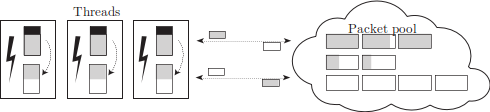
\includegraphics{figures/par_2}
  \caption[Γκρι πακέτα.]
    {Γκρι πακέτα. Κάθε νήμα ανταλλάσσει ένα άδειο πακέτο με
     ένα πακέτο αναφορών προς αντικείμενα προς εξιχνίαση. Η
     σήμανση γεμίζει ένα άδειο πακέτο με νέες αναφορές προς
     αντικείμενα προς εξιχνίαση: όταν αυτό γεμίσει, το νήμα
     το ανταλλάσσει με ένα καινούριο άδειο πακέτο από την
     καθολική δεξαμενή.}
  \label{fig:par_2}
\end{figure}

\subsection{Γκρι πακέτα}
Ο Ossia κ.ά \cite{DBLP:conf/pldi/OssiaBGKLO02}, καθώς και ο
Barabash κ.ά \cite{DBLP:journals/toplas/BarabashBGKLOOP05} 
παρατηρούν πώς η χρήση στοιβών
σήμανσης και κλοπής εργασίας είναι βέλτιστη όταν ο αριθμός των
νημάτων που συμμετέχουν στη συλλογή είναι γνωστός εξαρχής. Αυτό
δε συμβαίνει εάν κάθε νήμα τροποποιητής συμμετέχει πραγματοποιώντας
μια μικρή εργασία σε κάθε εκχώρηση. Επίσης παρατηρούν πώς είναι
πιθανόν δύσκολο για ένα νήμα να επιλέξει την καλύτερη ουρά από
την οποία θα κλέψει και ταυτόχρονα να εντοπίσει τον τερματισμό
της σήμανσης. Αντ'αυτού, εξισορροπούν το υπολογιστικό φορτίο
βάζοντας κάθε νήμα σήμανσης να ανταγωνίζεται για την απόκτηση
\textbf{πακέτων} αποτελούμενων από εργασίες σήμανσης. Το σύστημα
τους χρησιμοποιεί ένα σταθερό αριθμό από 1000 πακέτα των 512
εγγραφών το καθένα.

Κάθε νήμα σήμανσης χρησιμοποιεί δύο πακέτα: επεξεργάζεται
καταχωρίσεις από το πακέτο εισόδου και προσθέτει εργασίες 
σήμανσης στο πακέτο εξόδου. Ο όρος \textbf{γκρι πακέτα} οφείλεται 
στο γεγονός ότι τόσο το πακέτο εισόδου όσο και το πακέτο εξόδου
περιλαμβάνουν γκρι εγγραφές (αναφορές προς γκρι αντικείμενα)
σύμφωνα με την τριχρωματική αφαίρεση. Κάθε νήμα σήμανσης ανταγωνίζεται
με στόχο να αποκτήσει ένα πακέτο από μια καθολική δεξαμενή.
Αφού επεξεργασθεί όλες τις καταχωρίσεις ενός πακέτου, το επιστρέφει
στη δεξαμενή. Όταν το πακέτο εξόδου του είναι πλήρες, το επιστρέφει
στη δεξαμενή και παίρνει πίσω ένα φρέσκο πακέτο. Όπως φαίνεται
και στο σχήμα~\ref{fig:par2}, η κεντρική δεξαμενή αποτελείται
από τρεις συνδεδεμένες λίστες εκ των οποίων η πρώτη αποτελείται
από τελείως άδεια πακέτα, η δεύτερη από πακέτα σχεδόν μισογεμάτα
και η τρίτη από πακέτα σχεδόν γεμάτα. Τα νήματα προτιμούν την
τρίτη για την εισαγωγή ενός πακέτου εισόδου (\textproc{getInPacket})
και την πρώτη για την εξαγωγή ενός πακέτου εξόδου (\textproc{getOutPacket}).

Η τεχνική της παραλληλοποίησης της σήμανσης με γκρι πακέτα έχει
διάφορα πλεονεκτήματα. Ξεχωρίζοντας την είσοδο από την έξοδο,
ο Ossia κ.ά αποφεύγουν την εναλλαγή των ρόλων για τα πακέτα
ενός νήματος σήμανσης: το φορτίο εργασίας κατανέμεται ομοιόμορφα
στους επεξεργαστές καθώς ένας επεξεργαστής έχει την τάση να μην
καταναλώνει την έξοδό του. Καθώς ένα γκρι πακέτο περιλαμβάνει
μια ουρά από (αναφορές σε) αντικείμενα που θα επεξεργασθούν με
τη σειρά, προσφέρεται η δυνατότητα προφόρτωσης των επόμενων
αντικειμένων προς σήμανση.

Η τεχνική απαιτεί συγχρονισμό μόνο κατά τη μεταφορά των πακέτων
από και προς την καθολική δεξαμενή. Αυτό μειώνει τον αριθμό
των εντολών μνήμης \textbf{fence} που πρέπει να εισαχθούν από
το μεταγλωττιστή σε αρχιτεκτονικές με χαλαρό μοντέλο συνέπειας
μνήμης. Ένα νήμα χρειάζεται να εκτελέσει μία εντολή \textbf{fence}
μόνο όταν αποκτά πακέτα από την καθολική δεξαμενή ή επιστρέφει
πακέτα προς αυτή, και όχι μετά τη σήμανση και ώθηση ενός αντικειμένου
σε ένα πακέτο. Ο Ossia κ.ά χρησιμοποιούν ένα δίανυσμα από
\textbf{bits σήμανσης} όταν σαρώνουν συντηρητικά τις στοίβες
των νημάτων τροποποιητών προκειμένου να προσδιορίσουν αν μία
υποτιθέμενη αναφορά πραγματικά δείχνει προς κάποιο εκχωρηθέν
αντικείμενο. Τα bits σήμανσης χρησιμοποιούνται επίσης για το
συγχρονισμό μεταξύ των νημάτων τροποποιητών και των νημάτων
συλλεκτών. Οι εκχωρητές μνήμης χρησιμοποιούν τοπικούς απομονωτές
εκχώρησης. Κατά την υπερχείλιση ενός τοπικού απομονωτή εκχώρησης,
ο εκχωρητής εκτελεί μία εντολή \textbf{fence} και στη συνέχεια
θέτει σε λογικό 1 τα bits όλων των αντικείμενων που έχουν
εκχωρηθεί στον τοπικό απομονωτή, εξασφαλίζοντας με τον τρόπο
αυτό πώς οι αποθηκεύσεις που αφορούν την εκχώρηση και αρχικοποίηση
νέων αντικειμένων δεν προηγούνται των αποθηκεύσεων που αφορούν
την ενημέρωση των bits σήμανσης τους. Δύο ακόμη εντολές \textbf{fence}
είναι απαραίτητες. Πρώτον, όταν ένα νήμα εξιχνίασης αποκτά ένα
καινούριο πακέτο εισόδου, ελέγχει τα bits εκχώρησης όλων των
αντικειμένων του πακέτου και καταγράφει σε μία ιδιωτική δομή
δεδομένων για κάθε τέτοιο αντικείμενο αν είναι ασφαλής η
εξιχνίαση με ρίζα αυτό (αν το αντίστοιχο bit είναι σε λογικό
1). Στη συνέχεια το νήμα εκτελεί μία εντολή \textbf{fence}
πριν προχωρήσει στην εξιχνίαση με ρίζες τα ασφαλή αντικείμενα. 
Η εξιχνίαση με ρίζες τα μη ασφαλή αντικείμενα αναβάλλεται:
αυτά προστίθενται σε ένα πακέτο αναβολής, το οποίο κάποια
στιγμή αργότερα θα μεταφερθεί σε μία καθολική δεξαμενή
πακέτων αναβολής. Δεύτερον, ένα νήμα εξιχνίασης εκτελεί
μια εντολή \textbf{fence} όταν επιστρέφει το πακέτο εξόδου
του στην καθολική δεξαμενή (για να αποτρέψει την αναδιάταξη
αποθηκεύσεων στο πακέτο με την προσθήκη του πακέτου στην
καθολική δεξαμενή). Κατά την απόκτηση ενός πακέτου εισόδου
από την καθολική δεξαμενή υπάρχει μια εξάρτηση δεδομένων
μεταξύ της φόρτωσης του δείκτη προς το πακέτο και την πρόσβαση
στα περιεχόμενα και οι σύγχρονες αρχιτεκτονικές δεν αναδιατάσσουν
τις παραπάνω ενέργειες. Συνεπώς η εκτέλεση μιας εντολής
\textbf{fence} δεν είναι απαραίτητη σε αυτήν την περίπτωση.

Η τεχνική των γκρι πακέτων καθιστά εξαιρετικά απλή την
παρακολούθηση της κατάστασης. Κάθε καθολική δεξαμενή συσχετίζεται
με έναν καθολικό μετρητή του πλήθους των πακέτων της. Ο μετρητής
ενημερώνεται ατομικά κατά την προσθήκη ή αφαίρεση ενός
πακέτου από τη δεξαμενή. Η μέτρηση του πλήθους των πακέτων
είναι προσεγγιστική καθώς η μέτρηση μπορεί να διαβασθεί
αμέσως μετά την προσθήκη ενός πακέτου αλλά πριν την αύξηση
του μετρητή. Ωστόσο η συνθήκη τερματισμού απλώς ορίζει
ο μετρητής της καθολικής δεξαμενής άδειων πακέτων να ισούται
με το πλήθος των διαθέσιμων πακέτων. Η απόκτηση/επιστροφή
ενός πακέτου και η ενημέρωση του μετρητή της αντίστοιχης
καθολικής δεξαμενής δε χρειάζεται να είναι μία ενιαία
αδιαίρετη λειτουργία. Για να εξασφαλισθεί πώς ο μετρητής
κενών πακέτων δε θα μηδενισθεί προσωρινά, κάθε νήμα πρέπει
να αποκτήσει ένα καινούριο πακέτο εισόδου πριν επιστρέψει
το πακέτο εξόδου του στην καθολική δεξαμενή. 

\begin{algorithm}[H]
  \caption{Διαχείριση γκρι πακέτων}
  \label{alg:par4}
  \begin{algorithmic}[1]
    \State \textbf{shared} $fullPool$ \Comment{global pool of full packets}
    \State \textbf{shared} $halfFullPool$ \Comment{global pool of half full packets}
    \State \textbf{shared} $emptyPool$ \Comment{global pool of empty packets}
    \Statex
    \Function{getInPacket}{\null}
      \State \textbf{atomic}
      \State $inPacket \gets$ \Call{remove}{$fullPool$}
      \If{\Call{isEmpty}{$inPacket$}}
        \State \textbf{atomic}
        \State $inPacket \gets$ \Call{remove}{$halfFullPool$}
      \EndIf
      \If{\Call{isEmpty}{$inPacket$}}    
        \State $inPacket, outPacket \gets outPacket, inPacket$
      \EndIf
      \State \Return{\textbf{not} \Call{isEmpty}{$inPacket$}}
    \EndFunction
    \Statex
    \Procedure{testAndMarkSafe}{$packet$}
      \ForAll{$ref \; \textbf{in} \; packet$}
        \State \Call{safe}{$ref$} $\gets$ \Call{allocBit}{$ref$} $=\textbf{true}$ \Comment{private data structure}
      \EndFor
    \EndProcedure
    \Statex
    \Procedure{getOutPacket}{\null}
      \If{\Call{isFull}{$outPacket$}}
        \State \Call{generateWork}{\null}
      \EndIf
      \If{$outPacket = \textbf{null}$}
        \State \textbf{atomic}
        \State $outPacket \gets$ \Call{remove}{$emptyPool$}
      \EndIf
      \If{$outPacket = \textbf{null}$}
        \State \textbf{atomic}
        \State \Call{remove}{$halfFullPool$}
      \EndIf
      \If{$outPacket = \textbf{null}$}
        \If{\textbf{not} \Call{isFull}{$inPacket$}}    
          \State $inPacket, outPacket \gets outPacket, inPacket$
          \State \Return{\null}
        \EndIf  
      \EndIf
    \EndProcedure
    \Statex
    \Procedure{addOutPacket}{$ref$}
      \State \Call{getOutPacket}{\null}
      \If{$outPacket = \textbf{null}$ \textbf{or} \Call{isFull}{$outPacket$}}
        \State \Call{dirtyCard}{$ref$}
      \Else
        \State \Call{add}{$outPacket$, $ref$}
      \EndIf
    \EndProcedure
  \end{algorithmic}
\end{algorithm}

\begin{algorithm}[H]
  \caption{Παράλληλη εκχώρηση με χρήση γκρι πακέτων}
  \label{alg:par5}
  \begin{algorithmic}[1]
    \Function{sequentialAllocate}{$n$}
      \State $result \gets free$
      \State $newFree \gets result + n$
      \If{$newFree \leq labLimit$}
        \State $free \gets newFree$
        \State \Return{$result$}
      \EndIf
      \Statex
      \State /* local allocation buffer overflow */
      \State \textbf{fence}
      \ForAll{$obj \; \textbf{in} \; lab$}
        \State \Call{allocBit}{$obj$} $\gets \textbf{true}$
      \EndFor
      \State $lab, labLimit \gets$ \Call{newLab}{\null}
      \If{$lab = \textbf{null}$}
        \State \Return{\textbf{null}}
      \EndIf
      \State \Call{sequentialAllocate}{$n$} \Comment{signal 'Memory exhausted'}
    \EndFunction
  \end{algorithmic}
\end{algorithm}

\begin{algorithm}[H]
  \caption{Παράλληλη σήμανση με χρήση γκρι πακέτων}
  \label{alg:par6}
  \begin{algorithmic}[1]
    \State \textbf{shared} $fullPool$ \Comment{global pool of full packets}
    \Statex
    \Procedure{acquireWork}{\null}
      \If{\Call{isEmpty}{$inPacket$}}
        \If{\Call{getInPacket}{\null}}
          \State \Call{testAndMarkSafe}{$inPacket$}
          \State \textbf{fence}
        \EndIf
      \EndIf
    \EndProcedure
    \Statex
    \Procedure{performWork}{\null}
      \ForAll{$ref \; \textbf{in} \; inPacket$}
        \If{\Call{safe}{$ref$}}
          \ForAll{$fld \; \textbf{in} \; Pointers(ref)$}
            \State $child \gets *fld$
            \If{$child \neq \textbf{null}$ \textbf{and} \textbf{not} \Call{isMarked}{$child$}}
              \State \Call{setMarked}{$child$}
              \State \Call{addOutPacket}{$child$}
            \EndIf
          \EndFor   
        \Else
          \State \Call{addDeferredPacket}{$ref$} \Comment{defer tracing of unsafe objects}
        \EndIf
      \EndFor
    \EndProcedure
    \Statex
    \Procedure{generateWork}{\null}
      \State \textbf{fence}
      \State \Call{add}{$fullPool$, $outPacket$}
      \State $outPacket \gets \textbf{null}$
    \EndProcedure
  \end{algorithmic}
\end{algorithm}

\section{Παράλληλη αντιγραφή}
Η παραλληλοποίηση των αλγορίθμων συλλογής με αντιγραφή αντιμετωπίζει
λίγο πολύ τα ίδια ζητήματα με την παραλληλοποίηση των αλγορίθμων
συλλογής με σήμανση. Ωστόσο, παρότι η σήμανση ενός αντικειμένου
δύο φορές είναι αβλαβής, αυτό πρέπει να αντιγραφεί μόνο μία φορά.

\subsection{Διαμοιρασμός εργασίας ανάμεσα στους επεξεργαστές}
Οι Blelloch και Cheng \cite{DBLP:conf/pldi/BlellochC99, DBLP:conf/pldi/ChengB01}
παραλληλοποιούν την αντιγραφή στα πλαίσια της \textbf{επαναληπτικής
συλλογής}.

Οι επαναληπτικοί συλλέκτες είναι αυξητικοί ή ταυτόχρονοι συλλέκτες
που αντιγράφουν αντικείμενα την ώρα εκτέλεσης του τροποποιητή,
λαμβάνοντας ειδική φροντίδα για την επιδιόρθωση πεδίων που
εγγράφησαν από τον τροποποιητή κατά τη διάρκεια ενός κύκλου
συλλογής.

Κάθε νήμα αντιγραφής έχει τη δική του στοίβα εργασίας. Οι Blelloch
και Cheng ισχυρίζονται πώς οι στοίβες προσφέρουν ευκολότερο
συγχρονισμό μεταξύ των νημάτων αντιγραφής όπως επίσης και μικρότερο
ποσοστό κατακερματισμού από ότι οι ουρές Cheney. Το φορτίο εργασίας
εξισορροπείται βάζοντας τα νήματα αντιγραφής να μεταφέρουν περιοδικά
μονάδες εργασίας μεταξύ των τοπικών στοιβών και μιας καθολικής
στοίβας. Μια απλή μοιραζόμενη στοίβα απαιτεί το συγχρονισμό
μεταξύ των νημάτων που εκτελούν λειτουργίες ώθησης και εξώθησης
καταχωρίσεων. Δυστυχώς, δεν υπάρχει τρόπος ατομικής αύξησης
ή μείωσης του δείκτη στοίβας για την εισαγωγή και εξαγωγή ενός
στοιχείου με τη χρήση πρωταρχικών λειτουργιών όπως η \textproc{FetchAndAdd}
και η χρήση ενός κλειδώματος θα σειριοποιούσε την πρόσβαση στη
στοίβα. Η εντολή \textproc{FetchAndAdd} μπορεί ωστόσο να χρησιμοποιηθεί
ώστε να επιτραπεί σε πολλαπλά νήματα είτε να εισάγουν στοιχεία
στη στοίβα είτε να εξάγουν στοιχεία από τη στοίβα, καθώς
οι λειτουργίες αυτές έχουν ως τελικό αποτέλεσμα είτε την
αύξηση είτε τη μείωση του δείκτη στοίβας κατά περισσότερες
από μία θέσεις. Αφού ένα νήμα έχει πετύχει να μετακινήσει το
δείκτη στοίβας, πιθανώς κατά αρκετές θέσεις, μπορεί να διαβάσει
από η να γράψει στις θέσεις αυτές χωρίς τον κίνδυνο εμφάνισης
καταστάσεων συναγωνισμού.

Οι Cheng και Blelloch επιβάλλουν αυτού του είδους την πρόσβαση
στη μοιραζόμενη στοίβα χρησιμοποιώντας ένα μηχανισμό που
ονομάζουν \textbf{δωμάτια}. Υπάρχουν δύο δωμάτια: ένα ώθησης
και ένα εξώθησης και ανά πάσα χρονική στιγμή ένα εκ των δύο
πρέπει να είναι άδειο. Σε κάθε επανάληψη του βρόχου συλλογής,
ένα νήμα εισέρχεται αρχικά στο δωμάτιο εξώθησης και εκτελεί
ένα προκαθορισμένο αριθμό μονάδων εργασίας. Αποκτά αντικείμενα προς
σάρωση είτε από την τοπική του στοίβα είτε από την καθολική
στοίβα με χρήση της εντολής \textproc{FetchAndAdd}. Οι παραγόμενες
μονάδες εργασίας εισάγονται στην τοπική στοίβα. Στη συνέχεια
το νήμα εγκαταλείπει το δωμάτιο εξώθησης και περιμένει μέχρις
ότου και τα υπόλοιπα νήματα το έχουν εγκαταλείψει πριν προσπαθήσει
να εισέλθει στο δωμάτιο ώθησης. Το πρώτο νήμα που καταφέρνει
να εισέλθει κλείνει την πόρτα (μεταβλητή $gate$) ούτως ώστε
να απαγορευθεί η είσοδος στα υπόλοιπα νήματα. Ενώ βρίσκεται
μέσα στο δωμάτιο ώθησης, το νήμα αδειάζει πλήρως την τοπική
του στοίβα, μεταφέροντας όλα τα στοιχεία της στην καθολική
στοίβα, αφού πρώτα δεσμεύσει τον απαραίτητο χώρο με την εντολή
\textproc{FetchAndAdd}. Το τελευταίο νήμα που αποχωρεί από
το δωμάτιο ώθησης κλείνει την πύλη.

Το πρόβλημα του μηχανισμού είναι πώς ένας επεξεργαστής που
περιμένει για να εισέλθει στο δωμάτιο ώθησης υποχρεούται
να περιμένει μέχρις ότου όλοι οι επεξεργαστές που βρίσκονται
ήδη μέσα τελειώσουν τη σήμανση των αντικειμένων τους με
γκρι χρώμα. Ο χρόνος σήμανσης των αντικειμένων με γκρι
χρώμα είναι συγκρίσιμος με το χρόνο απόκτησης ή κατάθεσης
νέων μονάδων εργασίας και ένας επεξεργαστής που προσπαθεί
να εισέλθει στη φάση ώθησης πρέπει να περιμένει μέχρις ότου
όλοι οι υπόλοιποι επεξεργαστές που βρίσκονται στη φάση
εξώθησης τελειώσουν τη σήμανση των αντικειμένων τους με
γκρι χρώμα. Μεγάλες διακυμάνσεις στο χρόνο που χρειάζονται
οι επεξεργαστές για τη σήμανση των αντικειμένων τους με γκρι
χρώμα καθιστούν αυτό το χρόνο αδράνειας σημαντικό. Μια πιο
χαλαρή αφαίρεση θα επέτρεπε στους επεξεργαστές να εγκαταλείψουν
το δωμάτιο εξώθησης χωρίς να εισέλθουν στο δωμάτιο ώθησης.
Καθώς η σήμανση των αντικειμένων με γκρι χρώμα δε σχετίζεται
με τη μοιραζόμενη στοίβα, αυτή η εργασία μπορεί να πραγματοποιηθεί
εκτός των δωματίων. Αυτό αυξάνει σημαντικά την πιθανότητα
το δωμάτιο εξώθησης να είναι άδειο και συνεπώς ένα νήμα να
μπορέσει να εισέλθει στο δωμάτιο ώθησης.

Ο αρχικός μηχανισμός δωματίων των Cheng και Blelloch επιτρέπει
απλή ανίχνευση τερματισμού. Η τοπική στοίβα κάθε νήματος
είναι κενή όταν αυτό εγκαταλείπει το δωμάτιο ώθησης και επομένως
μένει στο τελευταίο νήμα που αποχωρεί να ελέγξει αν και
η καθολική μοιραζόμενη στοίβα είναι επίσης άδεια. Ωστόσο,
ο χαλαρός ορισμός του μηχανισμού των δωματίων επιτρέπει
στα νήματα να εργάζονται και εκτός δωματίων. Η υιοθέτηση αυτού
συνεπάγεται πώς η μοιραζόμενη στοίβα πρέπει να διατηρεί μία
καθολική μεταβλητή που μετράει πόσα νήματα έχουν δανεισθεί
αντικείμενα από αυτή. Το τελευταίο νήμα που αποχωρεί από το
δωμάτιο ώθησης ελέγχει ταυτόχρονα αν η μοιραζόμενη στοίβα είναι
κενή και ο καθολικός αυτός μετρητής μηδενικός.

\begin{algorithm}[H]
  \caption{Παράλληλη αντιγραφή (Cheng \& Blelloch)}
  \label{alg:par_7}
  \begin{algorithmic}[1]
    \State \textbf{shared} sharedStack \Comment{the shared stack of work}
    \State $myCopyStack[k]$ \Comment{local stack has k slots max}
    \State $sp \gets 0$
    \Statex
    \Procedure{run}{\null}
      \While{\textbf{not} \Call{terminated}{\null}}
        \State \Call{enterRoom}{\null} \Comment{enter pop room}
        \For{$i \gets 1 \; \textbf{to} \; k$}
          \If{\Call{isLocalStackEmpty}{\null}}
            \State \Call{acquireWork}{\null}
            \If{\Call{isLocalStackEmpty}{\null}}
              \State \textbf{break} 
            \EndIf
          \EndIf
          \State \Call{performWork}{\null}
        \EndFor
        \State \Call{generateWork}{\null}
        \If{\Call{exitRoom}{\null}} \Comment{leave push room}
          \State \Call{terminate}{\null}
        \EndIf
     \EndWhile
   \EndProcedure
   \Statex
   \Procedure{acquireWork}{\null} \Comment{move work from shared stack}
     \State \Call{sharedPop}{\null}
   \EndProcedure
   \Statex
   \Procedure{performWork}{\null}
     \State $ref \gets$ \Call{localPop}{\null}
     \State \Call{scan}{$ref$} \Comment{see algorithm~\ref{alg:cop_2}}
   \EndProcedure
   \Statex
   \Procedure{generateWork}{\null} \Comment{move work to shared stack}
     \State \Call{sharedPush}{\null}
   \EndProcedure
   \Statex
   \Function{isLocalStackEmpty}{\null}
     \State \Return{$sp=0$}
   \EndFunction
   \Statex
   \Procedure{localPush}{$ref$}
     \State $myCopyStack[sp++] \gets ref$
   \EndProcedure
   \Statex
   \Function{localPop}{\null}
     \Return{$myCopyStack[--sp]$}
   \EndFunction
   \Statex
   \Procedure{sharedPop}{\null} \Comment{move work from shared stack}
     \State $cursor \gets$ \Call{FetchAndAdd}{$\&sharedStack$, $1$} \Comment{try to grab from shared stack} 
     \If{$cursor > stackLimit$} \Comment{shared stack empty}
       \State \Call{FetchAndAdd}{$\&sharedStack$, $-1$} \Comment{readjust stack}
     \Else
       \State $myCopyStack[sp++] \gets cursor[0]$ \Comment{move work to local stack}
     \EndIf
   \EndProcedure
   \Statex
   \Procedure{sharedPush}{\null} \Comment{move work to shared stack}
     \State $cursor \gets$ \Call{FetchAndAdd}{$\&sharedStack$, $-sp$} $-sp$
     \For{$i \gets 0 \; \textbf{to} \; sp-1$}
       \State $cursor[i] \gets myCopyStack[i]$
     \EndFor
     \State $sp \gets 0$
   \EndProcedure
  \end{algorithmic}
\end{algorithm}

\begin{algorithm}[H]
  \caption{Συγχρονισμός λειτουργιών ώθησης/εξώθησης με δωμάτια}
  \label{alg:par_8}
  \begin{algorithmic}[1]
    \State \textbf{shared} $gate \gets OPEN$
    \State \textbf{shared} $popClients$ \Comment{number of clients currently in the pop room}
    \State \textbf{shared} $pushClients$ \Comment{number of clients currently in the push room}
    \Statex
    \Procedure{enterRoom}{\null}
      \While{$gate \neq OPEN$} \Comment{do nothing:wait}
      \EndWhile
      \State \Call{FetchAndAdd}{$\&popClients$, $1$} \Comment{try to start popping}
      \While{$gate \neq OPEN$}
        \State \Call{FetchAndAdd}{$\&popClients$, $-1$} \Comment{back out since did not succeed}
         \While{$gate \neq OPEN$} \Comment{do nothing:wait}
         \EndWhile
         \State \Call{FetchAndAdd}{$\&popClients$, $1$} \Comment{try again}
      \EndWhile
    \EndProcedure
    \Statex
    \Procedure{transitionRooms}{\null}
      \State $gate \gets CLOSED$
      \State \Call{FetchAndAdd}{$\&pushClients$, $1$} \Comment{move from popping to pushing}
      \State \Call{FetchAndAdd}{$\&popClients$, $-1$}
      \While{$popClients > 0$} \Comment{can't start pushing until none other popping}
      \EndWhile
    \EndProcedure
    \Statex
    \Procedure{exitRoom}{\null}
      \State $pushers \gets$ \Call{FetchAndAdd}{$\&pushClients$, $-1$} $-1$ \Comment{stop pushing}
      \If{$pushers = 0$} \Comment{I was last in room: check termination}
        \If{\Call{isEmpty}{$sharedStack$}}
          \State $gate \gets OPEN$
          \State \Return{\textbf{true}}
        \Else
          \State $gate \gets OPEN$
          \State \Return{\textbf{false}}
        \EndIf
      \EndIf
    \EndProcedure
  \end{algorithmic}
\end{algorithm}

\subsection{Αντιγράφοντας αντικείμενα παράλληλα}
Για να εξασφαλισθεί πώς μόνο ένα νήμα αντιγράφει ένα αντικείμενο,
τα νήματα πρέπει να συναγωνισθούν ώστε να αντιγράψουν ένα αντικείμενο
και να εγκαταστήσουν τη διεύθυνση προώθησης στην επικεφαλίδα
του παλαιού του αντιγράφου. Ο τρόπος αντιγραφής ενός αντικειμένου
από τα νήματα εξαρτάται από το εάν αυτά μοιράζονται μια μοναδική
περιοχή εκχώρησης μνήμης. Στην περίπτωση αυτή, τα νήματα αποφεύγουν
ορισμένη σπατάλη πληρώνοντας όμως το κόστος της χρήσης μιας
ατομικής λειτουργίας για εκχώρηση. Σε αυτήν την περίπτωση, οι
Blelloch και Cheng \cite{DBLP:conf/pldi/BlellochC99} θέτουν
να νήματα σε ανταγωνισμό για την εγγραφή μιας ειδικής τιμής
'busy' στην λέξη της επικεφαλίδας του αντικειμένου όπου θα
αποθηκευθεί η διεύθυνση προώθησης αυτού. Το νήμα νικητής αντιγράφει
το αντικείμενο πριν αποθηκεύσει τη διεύθυνση προώθησης, ενώ
τα νήματα ηττημένοι πρέπει να σπινάρουν μέχρις ότου παρατηρήσουν
μία έγκυρη διεύθυνση. Εναλλακτικά, αν κάθε νήμα γνωρίζει εξαρχής
σε ποια θέση θα αντιγράψει ένα αντικείμενο (για παράδειγμα
επειδή θα το αντιγράψει σε έναν τοπικό απομονωτή εκχώηρησης),
είναι τα νήματα να ανταγωνίζονται για να εγγράψουν ατομικά
τη διεύθυνση προώθησης προτού αντιγράψουν το αντικείμενο.

Ο συλλέκτης της Flood κ.ά \cite{DBLP:conf/jvm/FloodDSZ01} στον
οποίο αναφερθήκαμε προηγουμένως είναι γενεαλογικός. Η παλαιά
γενεά διαχειρίζεται από συλλογή με σήμανση και συμπύκνωση και
η νέα γενεά από συλλογή με αντιγραφή. Είδαμε παραπάνω τον
τρόπο με τον οποίο παραλληλοποιούν τη φάση της σήμανσης.
Εξετάζουμε τώρα πώς παραλληλοποιούν την αντιγραφή. Διπλά-τερματισμένες
κλεπτόμενες ουρές χρησιμοποιούνται και εδώ για τη διαχείριση
των αντικειμένων που πρόκειται να σαρωθούν. Ωστόσο, η παράλληλη αντιγραφή αντιμετωπίζει δύο
προβλήματα άγνωστα στην παράλληλη σήμανση: πρώτον, είναι επιθυμητή
η ελαχιστοποίηση του ανταγωνισμού για την εκχώρηση μνήμης όπου
θα αντιγραφεί ένα αντικείμενο και δεύτερον ένα ζωντανό αντικείμενο
πρέπει να αντιγραφεί μόνο μία φορά. Ο ανταγωνισμός για την
εκχώρηση μνήμης ελαχιστοποιείται με τη χρήση τοπικών απομονωτών
εκχώρησης για κάθε νήμα, τόσο για την αντιγραφή στους χώρους
επιζώντων στη νέα γενεά όσο και για την προαγωγή στην παλαιά
γενεά. Για να αντιγράψει ένα αντικείμενο, ένα νήμα πραγματοποιεί
μια υποθετική εκχώρηση στον τοπικό του απομονωτή εκχώρησης
και στη συνέχεια επιχειρεί μια πράξη \textproc{CompareAndSwap}
στον δείκτη προώθησης. Αν η τελευταία πετύχει, το νήμα αντιγράφει
το αντικείμενο. Αν όχι, επιστρέφει την τιμή του δείκτη προώθησης
που εγκατέστησε το νήμα νικητής.

\begin{figure}[H]
  \centering
  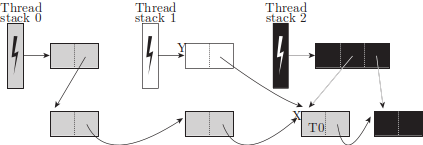
\includegraphics{figures/par_3}
  \caption[Εξιχνίαση κυρίαρχου νήματος.]
    {Εξιχνίαση κυρίαρχου νήματος. Τα νήματα 0 έως 2 με χρώμα
     μαύρο γκρι και άσπρο αντίστοιχα, έχουν εξιχνιάσει ένα
     γράφο αντικειμένων. Το χρώμα κάθε αντικειμένου υποδεικνύει
     τον επεξεργαστή στη μνήμη του οποίου θα αντιγραφεί. Το
     πρώτο πεδίο κάθε αντικειμένου είναι η επικεφαλίδα του.
     Το νήμα $T0$ είναι αυτό που τελευταίο κλείδωσε το αντικείμενο
     $X$.}
  \label{fig:par_3}
\end{figure}

 Ο διαχειριστής μνήμης του Ogasawara \cite{DBLP:conf/oopsla/Ogasawara09}
 λαμβάνει υπόψη την μη ομοιόμορφη προσπέλαση μνήμης και
 διαιρεί το σωρό σε τμήματα με μία ή περισσότερες σελίδες
 και κάθε τμήμα απεικονίζεται με έναν επεξεργαστή. Ο εκχωρητής
 μνήμης, ο οποίος χρησιμοποιείται τόσο από τα νήματα τροποποιητές
 όσο και από τα νήματα συλλέκτες προτιμά να εκχωρεί μπλοκ από
 τη μνήμη του προτιμώμενου επεξεργαστή. Για ένα νήμα τροποποιητή,
 αυτός ταυτίζεται με τον επεξεργαστή στον οποίο εκτελείται το
 νήμα. Τα νήματα συλλέκτες προσπαθούν πάντοτε να αντιγράψουν
 ζωντανά αντικείμενα σε σελίδες μνήμης που σχετίζονται με τον
 προτιμώμενο επεξεργαστή των τελευταίων. Καθώς το νήμα στο
 οποίο εκχωρήθηκε ένα αντικείμενο δεν είναι απαραίτητα και το
 νήμα που το χρησιμοποιεί περισσότερο συχνά, ο συλλέκτης
 χρησιμοποιεί πληροφορία \textbf{κυρίαρχου νήματος} για να
 προσδιορίζει τον προτιμώμενο επεξεργαστή κάθε αντικειμένου.
 Πρώτον, ο προτιμώμενος επεξεργαστής αντικειμένων προς τα οποία
 υπάρχουν άμεσες αναφορές από τη στοίβα ενός νήματος τροποποιητή
 θα είναι ο επεξεργαστής στον οποίο το νήμα εκτελέσθηκε για
 τελευταία φορά. Αυτό πιθανόν να δημιουργεί την απαίτηση τα
 νήματα να ενημερώνουν περιοδικά την ταυτότητα του προτιμώμενου
 επεξεργαστή τους. Δεύτερον, ο συλλέκτης μπορεί να χρησιμοποιήσει
 πληροφορίες σχετικές με το κλείδωμα αντικειμένων για να ταυτοποιήσει
 το \textbf{κυρίαρχο νήμα}. Οι μηχανισμοί κλειδωμάτων συχνά
 αποθηκεύουν την ταυτότητα του νήματος που έχει κλειδώσει ένα
 αντικείμενο σε μια λέξη στην επικεφαλίδα του αντικειμένου.
 Παρότι με αυτόν τον τρόπο ταυτοποιείται το νήμα (και συνεπώς
 και ο αντίστοιχος επεξεργαστής) που τελευταίο κλείδωσε το
 αντικείμενο, η προσέγγιση αυτή φαντάζει αρκετή καθώς τα
 περισσότερα αντικείμενα δεν ξεφεύγουν ποτέ από το νήμα στο
 οποίο εκχωρήθηκαν. Τέλος, ο συλλέκτης μπορεί να διαδώσει
 την ταυτότητα του προτιμώμενου επεξεργαστή από αντικείμενα
 γονείς σε αντικείμενα παιδιά.
  
 \subsection{Ξεχωριστοί ημιχώροι-από και ημιχώροι-προς}
 Η συλλογή με αντιγραφή από τη φύση
 \subsection{Σωροί οργανωμένοι κατά μπλοκ}
 Μία προσέγγιση είναι να υπερ-διαμερισθεί ο χώρος-προς και στη
 συνέχεια να νήματα να τεθούν σε ανταγωνισμό για την απόκτηση
 μπλοκ σάρωσης και αντιγραφής. Ο Imai κ.ά \cite{DBLP:journals/tpds/ImaiT93}
 διαιρούν το σωρό σε \textbf{κομμάτια (chunks)} σταθερού μεγέθους
 και παρέχουν σε κάθε νήμα τα δικά του κομμάτια σάρωσης
 και αντιγραφής επιζώντων αντικειμένων. Όταν το κομμάτι αντιγραφής
 ενός νήματος γεμίσει, αυτό μεταφέρεται σε μια καθολική δεξαμενή
 και τα ανενεργά νήματα ανταγωνίζονται για την απόκτηση και
 σάρωση του και το αρχικό νήμα αποκτά ένα καινούριο κομμάτι
 από το διαχειριστή ελεύθερων κομματιών.

 Δύο μηχανισμοί χρησιμοποιούνται για την εξισορρόπηση του φορτίου
 εργασίας. Αρχικά, τα κομμάτια αντιγραφής (τα οποία ονομάζουν
 μονάδες επέκτασης σωρού) είναι σχετικά μικρά (256 λέξεις). Δεύτερον,
 κάθε κομμάτι διαιρείται σε μικρότερα \textbf{μπλοκ} (τα οποία
 ονομάζουν μονάδες κατανομής φορτίου), με τυπικό μέγεθος 32 λέξεις.
 Κάθε νήμα προσφέρεται να παραχωρήσει μερικά από τα μη σαρωμένα
 μπλοκ του οποτεδήποτε χρειάζεται ένα νέο μπλοκ σάρωσης.  
 
 \section{Παράλληλη εκκαθάριση}
 Eξετάζουμε τώρα πώς μπορούν να παραλληλοποιηθούν οι φάσεις
 της εκκαθάρισης και της συμπύκνωσης. Και οι δύο φάσεις έχουν την
 ιδιότητα πώς η εξιχνίαση έχει ολοκληρωθεί και τα ζωντανά αντικείμενα
 του σωρού εντοπισθεί. Επίσης και οι δύο είναι εγγενώς παραλληλοποιήσιμες.

 Η παραλληλοποίηση της εκκαθάρισης μπορεί να επιτευχθεί είτε διαμερίζοντας
 στατικά το σωρό σε συνεχόμενες περιοχές, είτε υπερ-διαμερίζοντας
 τον σε μπλοκ και αφήνοντας να νήματα να ανταγωνίζονται για την
 εκκαθάριση ενός μπλοκ σε μία καθολική ελεύθερη λίστα μπλοκ. Ωστόσο,
 με την υιοθέτηση αυτής της απλής στρατηγικής είναι πιθανόν η ελεύθερη
 λίστα να καταστεί σημείο συμφόρησης και η συλλογή να σειριοποιηθεί.
 Ευτυχώς όμως σε ένα τέτοιου είδους παράλληλο σύστημα, κάθε επεξεργαστής
 διατηρεί συνήθως τοπικές ξεχωριστές ελεύθερες λίστες με μπλοκ
 διαφορετικών μεγεθών για την εκχώρηση μνήμης και έτσι το πρόβλημα
 του ανταγωνισμού ανάγεται στο χειρισμό της επιστροφής ολόκληρων
 ελεύθερων μπλοκ σε έναν καθολικό εκχωρητή μπλοκ. Επιπλέον, η
 οκνηρή εκκαθάριση αποτελεί από τη φύση της μιας παράλληλη λύση
 στο πρόβλημα της εκκαθάρισης μερικώς γεμάτων μπλοκ η οποία εξισορροπεί
 τις εργασίες εκκαθάρισης σύμφωνα με τους ρυθμούς εκχώρησης μνήμης
 στα νήματα τροποποιητές.

 Το πρώτο και μοναδικό βήμα της φάσης εκκαθάρισης όταν η τελευταία
 πραγματοποιείται οκνηρώς είναι η ταυτοποίηση πλήρως άδειων μπλοκ
 και η επιστροφή τους στον εκχωρητή μπλοκ. Για να μειώσουν τον
 ανταγωνισμό μεταξύ των νημάτων εκκαθάρισης, ο Endo κ.ά \cite{DBLP:conf/sc/EndoTY97}
 παρέχουν σε κάθε ένα από αυτά έναν αριθμό από συνεχόμενα μπλοκ
 προς τοπική επεξεργασία. Ο συλλέκτης τους χρησιμοποιεί bitmap
 σήμανσης, τα οποία αποθηκεύονται στις επικεφαλίδες των μπλοκ,
 ξεχωριστά από αυτά. Αυτή η προσέγγιση καθιστά εύκολο τον προσδιορισμό
 του κατά πόσο ένα μπλοκ είναι τελείως κενό από ζωντανά αντικείμενα.
 Τα άδεια μπλοκ ταξινομούνται και συνενώνονται πριν επιστραφούν
 σε μια τοπική ελεύθερη λίστα. Τα μερικώς γεμάτα από ζωντανά
 αντικείμενα μπλοκ εισάγονται σε τοπικές ξεχωριστές λίστες ανάκτησης
 για μπλοκ ξεχωριστών μεγεθών προς μελλοντική οκνηρή εκκαθάριση
 από τα νήματα τροποποιητές. Μόλις ένας επεξεργαστής ολοκληρώσει
 την εκκαθάριση του τοπικού του συνόλου εκκαθάρισης, συγχωνεύει
 την ελεύθερη λίστα μπλοκ αυτού με την καθολική ελεύθερη λίστα
 μπλοκ. Η τελευταία ερώτηση που μένει να απαντηθεί αφορά στο
 τι κάνει ένα νήμα τροποποιητής στην περίπτωση που τόσο η τοπική
 λίστα ανάκτησης όσο και η καθολική δεξαμενή μπλοκ είναι άδειες.
 Μια λύση είναι να κλέψει ένα μπλοκ από ένα άλλο νήμα, κάτι που
 απαιτεί το συγχρονισμό της απόκτησης του επόμενου μπλοκ προς
 εκκαθάριση. Το κόστος αυτό δεν είναι μεγάλο αν αναλογισθεί κανείς
 πώς αφενός η απόκτηση ενός μπλοκ προς εκκαθάριση συμβαίνει πιο
 σπάνια από ότι η αίτηση για εκχώρηση μνήμης στο εσωτερικό ενός
 μπλοκ και αφετέρου ο ανταγωνισμός πολλών νημάτων για την απόκτηση
 ενός μπλοκ προς εκκαθάριση δεν αναμένεται να συμβαίνει συχνά
 στην πράξη.

 \section{Παράλληλη συμπύκνωση}
 Η παραλληλοποίηση αλγορίθμων συλλογής σκουπιδιών με σήμανση
 και συμπύκνωση αφορά στην παράλληλη σήμανση των ζωντανών αντικειμένων
 και στη συνέχεια στην παράλληλη μετακίνηση αυτών. Ωστόσο η παράλληλη
 ολισθαίνουσα συμπύκνωση είναι απλούστερη από την παράλληλη
 αντιγραφή, τουλάχιστον σε συνεχόμενους σωρούς. Για παράδειγμα,
 όταν τα ζωντανά αντικείμενα έχουν σημανθεί ο προορισμός των αντικειμένων
 που θα μετακινηθούν δεν αλλάζει: οι καταστάσεις συναγωνισμού
 επηρεάζουν την επίδοση και όχι τόσο την ορθότητα. Μετά τη
 φάση της σήμανσης, οι περισσότεροι συλλέκτες με σήμανση και
 συμπύκνωση απαιτούν δύο ή και περισσότερα περάσματα στο σωρό
 προκειμένου να προσδιορίσουν τη διεύθυνση πρoώθησης κάθε αντικειμένου,
 να ενημερώσουν τις αναφορές προς κάθε αντικείμενο και να μετακινήσουν
 τα αντικείμενα. Όπως είδαμε στο κεφάλαιο \ref{ch:mark-compact}
 διαφορετικοί αλγόριθμοι μπορεί να εκτελούν αυτές τις εργασίες
 με διαφορετική σειρά ή να συνδυάσουν την εκτέλεση δύο εργασιών
 σε ένα μόνο πέρασμα.

 Ο Flood κ.ά \cite{DBLP:conf/jvm/FloodDSZ01} χρησιμοποιούν παράλληλη
 σήμανση και παράλληλη συμπύκνωση για τη διαχείριση της παλαιάς
 γενεάς στον παράλληλο γενεαλογικό συλλέκτη της εικονικής τους
 μηχανής για τη γλώσσα Java. Ο συλλέκτης χρησιμοποιεί τρεις επιπλέον
 φάσεις μετά την ολοκλήρωση της παράλληλης σήμανσης για να
 \begin{inparaenum}[(i)]
 \item υπολογίσει διευθύνσεις προώθησης
 \item ενημερώσει αναφορές και
 \item μετακινήσει αντικείμενα
 \end{inparaenum}. Το ενδιαφέρον χαρακτηριστικό της σχεδίασης
 τους είναι πώς χρησιμοποιούν διαφορετική στρατηγική εξισορρόπησης
 φορτίου σε κάθε διαφορετική φάση συμπύκνωσης. Οι αλγόριθμοι
 συμπύκνωσης για μονοεπεξεργαστικά συστήματα πραγματοποιούν την
 ολίσθηση των ζωντανών αντικειμένων στο ένα άκρο του σωρού.
 Αν όμως υπάρχουν πολλαπλά νήματα συμπύκνωσης μετακινούν αντικείμενα
 παράλληλα, τότε απαιτείται προσοχή ούτως ώστε να αποτραπεί η
 εγγραφή δεδομένων ενός ζωντανού αντικειμένου από ένα νήμα
 συμπύκνωσης πριν τη μετακίνησή του αντικειμένου από ένα άλλο
 νήμα συμπύκνωσης. Για το λόγο αυτό, ο Flood κ.ά δε συμπυκνώνουν
 όλα τα αντικείμενα σε ένα πυκνό άκρο του σωρού, αλλά αντίθετα
 διαιρούν το σωρό σε περιοχές και αναθέτουν σε κάθε νήμα συμπύκνωσης
 τη δική του περιοχή. Κάθε νήμα συμπύκνωσης είναι υπεύθυνο για
 την ολίσθηση ζωντανών αντικειμένων μόνο στη δική του περιοχή.
 Επιπλέον, προκειμένου να μειωθεί ο (περιορισμένος) κατακερματισμός
 που μπορεί να προκύψει από τη χρήση αυτής της στρατηγικής
 διαμέρισης του σωρού, η κατεύθυνση ολίσθησης αντικειμένων
 εναλλάσσεται μεταξύ δύο διαδοχικών περιοχών. 

\begin{figure}[H]
  \centering
  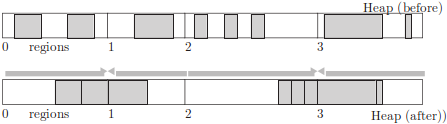
\includegraphics{figures/par_5}
  \caption
    [Διαίρεση του σωρού σε μία περιοχή ανά νήμα συμπύκνωσης
     και εναλλαγή της κατεύθυνσης ολίσθησης αντικειμένων μεταξύ
     δύο διαδοχικών νημάτων συμπύκνωσης.]
    {Διαίρεση του σωρού σε μία περιοχή ανά νήμα συμπύκνωσης
     και εναλλαγή της κατεύθυνσης ολίσθησης αντικειμένων μεταξύ
     δύο διαδοχικών νημάτων συμπύκνωσης.}
  \label{fig:par_5}
\end{figure}

Το πρώτο βήμα είναι η εγκατάσταση ενός δείκτη προώθησης στην
επικεφαλίδα κάθε ζωντανού αντικειμένου. Ο δείκτης αυτός θα
αποθηκεύει τη διεύθυνση στην οποία το αντικείμενο πρόκειται
να μετακινηθεί. Σε αυτή τη φάση, ο σωρός υπερ-διαμερίζεται
για να βελτιωθεί η εξισορρόπηση φορτίου. Ο χώρος διαιρείται
σε $M$ \textbf{μονάδες} ευθυγραμμισμένες με βάση τα αντικείμενα
και η κάθε μονάδα έχει σχεδόν το ίδιο μεγέθος. Ο Flood κ.ά υπολόγισαν
πώς μία καλή επιλογή για τον UltraSPARC διακομιστή είναι ο
αριθμός των χρησιμοποιούμενων μονάδων να είναι τετραπλάσιος
του αριθμού των νημάτων συμπύκνωσης ($M=4N$). Τα νήματα συμπύκνωσης
ανταγωνίζονται μεταξύ τους για την απόκτηση μονάδων και στη
συνέχεια υπολογίζουν τον όγκο των ζωντανών δεδομένων σε κάθε
μονάδα. Μάλιστα, για να διευκολυνθούν οι επόμενες φάσεις,
συνενώνουν γειτονικά σκουπίδια. Μόλις ο όγκος των ζωντανών
δεδομένων σε κάθε μονάδα γίνει γνωστός, ο σωρός μπορεί να 
διαιρεθεί σε $N$ \textbf{περιοχές} που η καθεμία περιλαμβάνει
σχεδόν τον ίδιο όγκο ζωντανών δεδομένων. Αυτές οι περιοχές
είναι ευθυγραμμισμένες με τις μονάδες της προηγούμενης φάσης.
Επίσης υπολογίζεται η διεύθυνση προορισμού για κάθε ζωντανό
αντικείμενο, λαμβάνοντας υπόψη την κατεύθυνση ολίσθησης σε
κάθε περιοχή. Τα νήματα συμπύκνωσης πλέον ανταγωνίζονται μεταξύ
τους για την απόκτηση μονάδων και εγκαθιστούν τους δείκτη προώθησης
σε κάθε ζωντανό αντικείμενο των μονάδων τους.

Η επόμενη φάση πραγματοποιεί την ενημέρωση των κατάλληλων αναφορών
με τις νέες διευθύνσεις των μετακινηθέντων αντικειμένων. Ως
συνήθως αυτό απαιτεί τη σάρωση στοιβών των νημάτων τροποποιητών,
των αναφορές σε αντικείμενα ενός υποχώρου του σωρού που είναι
αποθηκευμένες σε πεδία αντικειμένων εκτός της μονάδας καθώς
επίσης και των ζωντανών αντικειμένων αυτού του υποχώρου του
σωρού (για παράδειγμα στην παλαιά γενεά). Οποιαδήποτε κατάλληλη
στρατηγική διαμοιρασμού φορτίου μπορεί να χρησιμοποιηθεί. Ο
Flood κ.ά χρησιμοποιούν εκ νέου τη διαμέριση σε μονάδες για
τη σάρωση του προς συμπύκνωση υποχώρου του σωρού (της παλαιάς
γενεάς) παρότι η σάρωση της νέας γενεάς πραγματοποιείται ως
μια αδιαίρετη εργασία, δηλαδή σειριακά. Η τελευταία φάση μετακινεί
τα αντικείμενα. Ο Flood κ.ά αναθέτουν σε κάθε νήμα συμπύκνωσης
τη μετακίνηση αντικειμένων μιας περιοχής. Αυτή η προσέγγιση
εξισορροπεί το φόρτο εργασίας ομοιόμορφα μεταξύ των νημάτων
συμπύκνωσης, αφού οι περιοχές ορίσθηκαν ώστε να έχουν σχεδόν
τον ίδιο όγκο ζωντανών δεδομένων.

\begin{figure}[H]
  \centering
  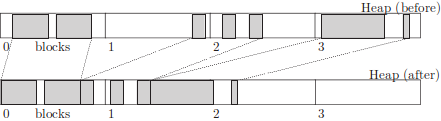
\includegraphics{figures/par_6}
  \caption
    [Συμπύκνωση με ολίσθηση μπλοκ.]
    {Συμπύκνωση με ολίσθηση μπλοκ. Ο Abuaiadh κ.ά ολισθαίνουν
     ολισθαίνουν ολόκληρα μπλοκ και όχι ξεχωριστά αντικείμενα.}
  \label{fig:par_6}
\end{figure}

Υπάρχουν δύο μειονεκτήματα όσον αφορά τον τρόπο που ο αλγόριθμος
συμπυκνώνει αντικείμενα. Πρώτον, πραγματοποιεί τρία περάσματα
στο σωρό. Δεύτερον, αντί να συμπυκνώσουν όλα τα ζωντανά αντικείμενα
στο ένα άκρο της παλαιάς γενεάς του σωρού, ο Flood κ.ά συμπυκνώνουν
την παλαιά γενεά σε $N$ πυκνά τμήματα, αφήνοντας $\lceil{\frac{N+1}{2}}\rceil$
κενά για εκχώρηση. Δε σπαταλάται χώρος σε κάθε συμπυκνωμένο τμήμα
εκτός ίσως για λόγους ευθυγράμμισης των αντικειμένων. Ωστόσο, αν
ο αριθμός των περιοχών ή νημάτων συμπύκνωσης είναι πολύ μεγάλος,
η εκχώρηση μεγάλων αντικειμένων στα νήματα τροποποιητές μπορεί
να καταστεί αδύνατη.

Ο Abuaiadh κ.ά \cite{DBLP:conf/oopsla/AbuaiadhOPS04} για να αντιμετωπίσουν
το πρώτο πρόβλημα υπολογίζουν μόνο και δεν αποθηκεύουν τις διευθύνσεις
προώθησης, χρησιμοποιώντας το bitmap σήμανσης και ένα διάνυσμα
μετατόπισης που αποθηκεύει τη νέα διεύθυνση του πρώτου ζωντανού
αντικειμένου σε κάθε μικρό μπλοκ του σωρού. Λύνουν το δεύτερο πρόβλημα
υπερ-διαμερίζοντας το σωρό σε έναν αριθμό σχετικά μεγάλες περιοχές.
Για παράδειγμα, προτείνουν το πλήθος των περιοχών να είναι τετραπλάσιο
του αριθμού των επεξεργαστών και η κάθε περιοχή να είναι τουλάχιστον
4 MB. Οι περιοχές του σωρού συμπυκνώνονται με τη σειρά. Tα νήματα
συμπύκνωσης ανταγωνίζονται για την απόκτηση μιας περιοχής χρησιμοιώντας
μια ατομική λειτουργία για να αυξήσουν έναν καθολικό μετρητή (ή
δείκτη). Αν η αύξηση είναι επιτυχής, το νήμα συμπύκνωσης έχει
αποκτήσει την περιοχή. Αν πάλι όχι, η συγκεκριμένη περιοχή βρίσκεται
στην κατοχή κάποιου άλλου νήματος συμπύκνωσης και το νήμα προσπαθεί
να αποκτήσει την επόμενη περιοχή. Ένας πίνακας αποθηκεύει δείκτες
προς την αρχή του ελεύθερου χώρου κάθε περιοχής. Αφού αποκτήσει
μια περιοχή για συμπύκνωση, ένα νήμα διεκδικεί μία περιοχή στην
οποία μπορεί να μετακινήσει αντικείμενα. Ένα νήμα αποκτά μια
περιοχή προσπαθώντας να γράψει την ειδική τιμή \textbf{null}
στο αντίστοιχο πεδίο του πίνακα. Τα νήματα συμπύκνωσης ποτέ δε
συμπυκνώνουν από ή προς μια περιοχή της οποίας ο αντίστοιχος
δείκτης στον πίνακα έχει την τιμή \textbf{null}, ενώ δε μεταφέρονται
αντικείμενα από κάποια περιοχή με μικρότερο αριθμό προς κάποια
περιοχή με μεγαλύτερο αριθμό. Η πρόοδος εξασφαλίζεται αφού ένα
νήμα μπορεί πάντοτε να συμπυκνώσει μια περιοχή στον εαυτό της.
Όταν ένα νήμα ολοκληρώσει τη συμπύκνωση μιας περιοχής, ενημερώνει
τον κατάλληλο δείκτη του πίνακα και στην περίπτωση που μια περιοχή
είναι γεμάτη, ο τελευταίος εξακολουθεί να έχει την τιμή \textbf{null}.

Ο Abuaiadh κ.ά εξερεύνησαν δύο τρόπους μετακίνησης αντικειμένων.
Η βέλτιστη συμπύκνωση με τον ελάχιστο κατακερματισμό προκύπτει
από την μετακίνηση ζωντανών αντικειμένων ξεχωριστά, όπως ακριβώς
περιγράφηκε πιο πάνω. Επειδή κάθε αντικείμενο ενός μπλοκ μετακινείται
σε μία θέση που εν μέρει προσδιορίζεται από το διάνυσμα μετατοπίσεων
για τον εν λόγω μπλοκ, τα αντικείμενα ενός μπλοκ δε διασκορπίζονται
μεταξύ δύο διαφορετικών περιοχών. Ο Abuaiadh κ.ά δοκίμασαν επίσης
να μειώσουν το χρόνο συμπύκνωσης θυσιάζοντας την ποιότητα της δια
μέσου της μετακίνησης ολόκληρων μπλοκ (256 bytes). Καθώς τα αντικείμενα
ενός χώρου μνήμης που εκχωρείται σειριακά έχουν την τάση να ζουν
και να πεθαίνουν σε συστάδες, ο Abuaiadh κ.ά υπολόγισαν πώς
η τεχνική αυτή μπορεί να μειώσει το συνολικό χρόνο συμπύκνωσης
κατά 20\% πληρώνοντας το κόστος της αύξησης του μεγέθους της
περιοχής συμπύκνωσης κατά ένα πολύ μικρό ποσοστό. Από την άλλη
πλευρά όμως, δεν είναι δύσκολη η επινόηση μιας περίπτωσης όπου
η τεχνική αυτή οδηγεί σε μηδενική συμπύκνωση.

Ο μηχανισμός υπολογισμού μόνο και όχι αποθήκευσης της διεύθυνσης
προώθησης ενός αντικειμένου υιοθετήθηκε αργότερα από τον αλγόριθμο
Compressor των Kermany και Petrank \cite{DBLP:conf/pldi/KermanyP06}.
Ο αλγόριθμος Compressor ωστόσο εισάγει κάποιες διαφορές. Πρώτον,
καθώς η δεύτερη φάση της συλλογής σαρώνει το bitmap σήμανσης,
υπολογίζει εκτός από το διάνυσμα μετατόπισης και ένα επιπλέον
βοηθητικό διάνυσμα, το οποίο δεικτοδοτείται από τις σελίδες προορισμού
των αντικειμένων. Σε κάθε θέση του βοηθητικού διανύσματος αποθηκεύεται
η αρχική διεύθυνση του πρώτου αντικειμένου που θα μετακινηθεί
στην αντίστοιχη σελίδα. Η συμπύκνωση καθεαυτή εκκινεί με την
ενημέρωση των ριζών.

Η δεύτερη διαφορά είναι πώς στη συνέχεια κάθε νήμα ανταγωνίζεται
για την απόκτηση μιας σελίδας-προς από το βοηθητικό διάνυσμα.
Μετά την επιτυχή προσπάθεια απόκτησης μιας σελίδας-προς, ένα
νήμα συμπύκνωσης αντιστοιχίζει την εικονική αυτή σελίδα σε μία
καινούρια φυσική σελίδα και ξεκινά να μεταφέρει αντικείμενα
με χρήση των διανυσμάτων σήμανσης και μετατόπισης και εκκινώντας
από τη διεύθυνση που υποδεικνύει το βοηθητικό διάνυσμα. Η απόκτηση
μιας νέας σελίδας-προς, στην οποία μπορεί να μεταφέρει αντικείμενα
επιτρέπει στον αλγόριθμο Compressor τη χρήση παράλληλων νημάτων
συμπύκνωσης. Εκ πρώτης όψεως, φαίνεται πώς ο Compressor είναι
αλγόριθμος συλλογής με αντιγραφή και όχι με σήμανση και εκκαθάριση.
Στην πραγματικότητα όμως πρόκειται για ένα συλλέκτη με σήμανση
και ολισθαίνουσα συμπύκνωση. Κάθε νήμα συμπύκνωσης διαχειρίζεται
κάθε ζεύγος από μια εικονική σελίδα-από και μια εικονική σελίδα-προς
με χρήση μίας φυσικής σελίδας μνήμης: όπως ακριβώς προσθέτει
μια αντιστοίχιση μεταξύ της εικονικής σελίδας-προς και μιας
καινούριας φυσικής σελίδας τη στιγμή της απόκτησης της σελίδας-προς,
με τον ίδιο τρόπο αφαιρεί μια αντιστοίχιση μεταξύ μιας εικονικής
σελίδας-από και της αντίστοιχης φυσικής σελίδας τη χρονική στιγμή
της ολοκλήρωσης της μεταφοράς των ζωντανών αντικειμένων από τη
σελίδα-προς.
 
Αυτή η σχεδίαση ελαχιστοποιεί την επιβάρυνση εξαιτίας του συγχρονισμού
των νημάτων συμπύκνωσης. Μόνο η προσπάθεια απόκτησης μιας σελίδας-προς
από το βοηθητικό διάνυσμα εκτελείται συγχρονισμένα από ένα νήμα
συμπύκνωσης. Αν η προσπάθεια είναι ανεπιτυχής, το νήμα προσπαθεί
να αποκτήσει τη σελίδα-προς στην οποία αντιστοιχεί η επόμενη
θέση του βοηθητικού διανύσματος. Ο τερματισμός της συμπύκνωσης
είναι εξίσου απλός: η εκτέλεση ενός νήματος συμπύκνωσης ολοκληρώνεται
όταν αυτό έχει εξετάσει και την τελευταία θέση του βοηθητικού
διανύσματος. 

\section{Ανακεφαλαίωση και θέματα προς εξέταση}
\subsection{Ορολογία}
Οι δημοσιεύσεις του 20ού αιώνα χρησιμοποιούν αυθαίρετα και
αδιακρίτως τους όρους παράλληλος, ταυτόχρονος και πραγματικού-χρόνου.
Από το 2000 ωστόσο, οι ερευνητές έχουν υιοθετήσει μία συνεπή
χρήση των όρων. Ένας παράλληλος συλλέκτης σκουπιδιών είναι ένας
συλλέκτης που χρησιμοποιεί πολλά νήματα συλλογής, τα οποία
εκτελούνται παράλληλα. Ο κόσμος μπορεί να διακόπτεται αλλά και
να μην διακόπτεται κατά τη διάρκεια εκτέλεσης των παράλληλων
νημάτων συλλεκτών. Με τον ίδιο τρόπο που είναι επιθυμητό να
επιτρέπεται σε πολλαπλά νήματα τροποποιητές να κάνουν χρήση
όλων των παράλληλων πόρων, η επίτρεψη της παράλληλης συλλογής
όταν η αρχιτεκτονική το επιτρέπει αποτελεί συνετή πράξη.

\subsection{Αξίζει η παραλληλοποίηση;}
Λαμβάνοντας υπόψη το νόμο του Amdahl \footnote{Ο νόμος του Amdahl
δηλώνει πώς η επιτάχυνση που προκύπτει από την παραλληλοποίηση
ενός προγράμματος εξαρτάται από το} προκύπτει το εύλογο ερώτημα
αν υπάρχει επαρκής δουλειά προς παραλληλοποίηση. Είναι εύκολο
να φανταστεί κανείς σενάρια που δεν προσφέρουν ευκαιρίες για
παραλληλοποίηση: ένα συνηθισμένο παράδειγμα τέτοιου σεναρίου
αποτελεί η εξιχνίαση μιας απλής συνδεδεμένης λίστας. Όπως
παρατηρεί ο Siebert \cite{DBLP:conf/iwmm/Siebert08}, υπάρχουν
πολλές ενδείξεις πώς οι πραγματικές εφαρμογές χρησιμοποιούν
ένα πολύ πιο πλούσιο ρεπερτόριο από δομές δεδομένων προσφέροντας
δυνατότητες παραλληλοποίησης υψηλού βαθμού. Εκτός από τη σήμανση,
οι υπόλοιπες δραστηριότητες της συλλογής σκουπιδιών προσφέρουν
εμφανώς περισσότερες δυνατότητες εκμετάλλευσης του παράλληλου
υλικού. Για παράδειγμα, η εκκαθάριση και η συμπύκνωση είναι
εγγενώς παραλληλοποιήσιμες διαδικασίες (παρότι η δεύτερη απαιτεί
λίγη παραπάνω προσοχή). Ακόμη και στη φάση της σήμανσης ωστόσο,
οι στοίβες και τα ενθυμούμενα σύνολα των νημάτων τροποποιητών
δύνανται να σαρώνονται παράλληλα και με μία μικρή επιβάρυνση
συγχρονισμού. Η παράλληλη εξιχνίαση του γράφου αντικειμένων
απαιτεί προσεκτικό σχεδιασμό όσον αφορά το χειρισμό των λιστών
εργασιών ούτως ώστε να περιορισθεί το κόστος συγχρονισμού και
ταυτόχρονα οι παράλληλοι πόροι του συστήματος να χρησιμοποιούνται
όσο το δυνατόν αποδοτικότερα.

\subsection{Στρατηγικές εξισορρόπησης φορτίου εργασίας}
Η αποδοτική παραλληλοποίηση της συλλογής απαιτεί προσεκτικό
συμβιβασμό μεταξύ της εξισορρόπησης του φορτίου εργασίας
μεταξύ των επεξεργαστών και του απαραίτητου συγχρονισμού.
Η εξισορρόπηση του φορτίου εργασίας εξασφαλίζει την αποτροπή
μιας κατάστασης όπου ορισμένοι επεξεργαστές εκτελούν όλες
τις εργασίες και κάποιοι άλλοι είναι αδρανείς. Ο συγχρονισμός
είναι απαραίτητος καθώς εξασφαλίζει την ακεραίοτητα τόσο των
ιδιωτικών δομών δεδομένων των νημάτων όσο και των καθολικών
δομών δεδομένων του σωρού.
 
Η γενική λύση ορίζει την ανάθεση στα νήματα συλλογής κβάντων
εργασίας τα οποία μπορούν να εκτελέσουν χωρίς περαιτέρω
συγχρονισμό. Η φθηνότερη λύση όσον αφορά το κόστος συγχρονισμού
αφορά τη στατική διαίρεση της εργασίας είτε κατά την εκκίνηση
του προγράμματος είτε ακριβώς πριν από κάθε κύκλο συλλογής.
Στην περίπτωση αυτή απαιτείται συντονισμός μεταξύ των παράλληλων
νημάτων απαιτείται μόνο για τον εντοπισμό του τερματισμού μιας
φάσης συλλογής. Ωστόσο η στατική διαμέριση μπορεί να μην οδηγήσει
σε ικανοποιητική εξισορρόπηση του φορτίου εργασίας. Το φορτίο
εργασίας μπορεί να εξισορροπισθεί επίσης υπερ-διαμερίζοντας
τη διαθέσιμη εργασία σε υποεργασίες και θέτοντας τα παράλληλα
νήματα να ανταγωνίζονται μεταξύ τους για την απόκτηση κβάντων
εργασίας από μια καθολική δεξαμενή καθώς και να επιστρέφουν
καινούρια κβάντα εργασίας σε αυτή. Η δεύτερη προσέγγιση έχει
εμφανώς μεγαλύτερο κόστος συγχρονισμού.

Συχνά βέβαια είναι δυνατή η εφαρμογή διαφορετικών στρατηγικών
εξισορρόπησης του φορτίου εργασιών σε διαφορετικές φάσεις ενός
κύκλου συλλογής. Η πληροφορία που γίνεται διαθέσιμη μετά το
πέρας μιας φάσης (συνήθως της φάσης σήμανσης) μπορεί να χρησιμοποιηθεί
προκειμένου να εκτιμηθεί μια δίκαιη διαίρεση της εργασίας των
επόμενων φάσεων ανάμεσα στα παράλληλα νήματα.
 
\subsection{Χειρισμός εξιχνίασης}
Η εξιχνίαση του σωρού περιλαμβάνει την κατανάλωση εργασίας
και την παραγωγή περαιτέρω εργασίας. Μια δομή δεδομένων, όπως
μια στοίβα ή μια ουρά είναι απαραίτητη για την καταγραφή
της εργασίας. Μια μοναδική, διαμοιραζόμενη δομή θα οδηγούσε
σε υψηλό κόστος συγχρονισμού και συνεπώς θα πρέπει να νήματα
να διατηρούν τις δικές τους ιδιωτικές δομές δεδομένων. Ωστόσο
η εξισορρόπηση του φορτίου εργασίας απαιτεί την ύπαρξη ενός
μηχανισμού μεταφοράς μονάδων εργασίας μεταξύ των νημάτων.
Η πρώτη απόφαση αφορά στην επιλογή του μηχανισμού. Δομές
δεδομένων που υποστηρίζουν κλοπή εργασίας μπορούν να χρησιμοποιηθούν
ώστε να επιτραπεί η μεταφορά μονάδων εργασίας μεταξύ των νημάτων.
Η ιδέα είναι η κοινή λειτουργία (ώθηση και εξώθηση στοιχείων
κατά την εξιχνίαση) να καταστεί όσο φθηνότερη (δηλαδή ασυγχρόνιστη)
γίνεται ενώ ταυτόχρονα επιτρέπονται λιγότερο συχνές λειτουργίες
(ασφαλής μεταφορά εργασίας μεταξύ των νημάτων). Ο Endo κ.ά
\cite{DBLP:conf/sc/EndoTY97} παρέχουν σε κάθε νήμα μία ιδιωτική
στοίβα και μία κλεπτόμενη ουρά εργασίας, ενώ ο Flood κ.ά
\cite{DBLP:conf/jvm/FloodDSZ01}
χρησιμοποιούν απλώς μια διπλά-τερματισμένη ουρά τόσο για τη
σήμανση όσο και για την κλοπή. Η τεχνική των γκρι πακέτων
\cite{DBLP:conf/pldi/OssiaBGKLO02}
διατηρεί μια καθολική δεξαμενή πακέτων εργασιών. Εδώ κάθε
νήμα ανταγωνίζεται για την απόκτηση ενός πακέτου εργασίας
από την καθολική δεξαμενή και επιστρέφει καινούρια εργασία
σε αυτή μέσω ενός φρέσκου πακέτου. Οι Cheng και Blelloch
\cite{DBLP:conf/pldi/ChengB01} λύνουν το πρόβλημα του συγχρονισμού των λειτουργιών
ώθησης και εξώθησης στοίβας χωρίζοντας την εξιχνίαση σε δύο
φάσεις που ονομάζουν δωμάτια. Η απλούστερη εκδοχή του αλγορίθμου
τους ορίζει πώς όλα τα νήματα βρίσκονται είτε στο δωμάτιο
ώθησης είτε στο δωμάτιο εξώθησης. Σε κάθε περίπτωση όλα τα
νήματα επιθυμούν να μετακινήσουν το δείκτη στοίβας προς την
ίδια κατεύθυνση και αυτό έχει ως αποτέλεσμα τη δυνατότητα
χρήσης μιας ατομικής λειτουργίας όπως η \textproc{FetchAndAdd}.

Η δεύτερη απόφαση αφορά το μέγεθος και τον τρόπο της μεταφερόμενης
εργασίας. Η ελάχιστη μεταφερόμενη μονάδα εργασίας είναι ένα
στοιχείο της στοίβας. Ωστόσο, η χρήση μικρών δομών δεδομένων
μπορεί να οδηγήσει στη διακίνηση μεγαλύτερου όγκου δεδομένων
μεταξύ των νημάτων. Στον παράλληλο, ταυτόχρονο και πραγματικού
χρόνου συλλέκτη του, o Siebert \cite{DBLP:conf/iwmm/Siebert10}
επιτρέπει σε έναν αδρανή επεξεργαστή να κλέψει ολόκληρη τη
δουλειά από έναν άλλον επεξεργαστή. Αυτή η απόφαση είναι συνετή
μόνο αν η περίπτωση να ξεμείνουν και οι υπόλοιποι επεξεργαστές
από δουλειά περίπου την ίδια χρονική στιγμή είναι σχεδόν
απίθανη. Μια συνήθης πρακτική είναι να μεταφέρεται ένα ενδιάμεσο
μέγεθος εργασίας ανάμεσα στα νήματα. Με τη χρήση γκρι πακέτων
σταθερού μεγέθους αυτό γίνεται αυτόματα. Μια άλλη επιλογή
είναι η μεταφορά της μισής ιδιωτικής στοίβας σήμανσης ενός
νήματος. Αν οι ιδιωτικές στοίβες σήμανσης έχουν σταθερό
μέγεθος, τότε απαιτείται και ένας μηχανισμός χειρισμού της
υπερχείλισης. Και αυτή η περίπτωση αντιμετωπίζεται αυτόματα
από την τεχνική των γκρι πακέτων: όταν ένα γεμάτο πακέτο
εξόδου γεμίζει μεταφέρεται στην καθολική και δεξαμενή και
λαμβάνεται ένα άδειο πακέτο από αυτή. Ο Flood κ.ά 
\cite{DBLP:conf/jvm/FloodDSZ01} χειρίζονται την υπερχείλιση
μέσω αντικειμένων κλάσεων στη γλώσσα Java, πληρώνοντας ένα
μικρό κόστος σε χώρο για κάθε κλάση.

Στο επίκεντρο της σχεδίασης των παραπάνω αλγορίθμων είναι ο
επεξεργαστής. Στρατηγικές όπου στο επίκεντρο της σχεδίασης
είναι η μνήμη και οι οποίες λαμβάνουν υπόψη τις θέσεις των
αντικειμένων στο σωρό είναι πιο συνήθεις σε αλγορίθμους για
συλλογή με παράλληλη αντιγραφή, όπου οι λίστες εργασίες
οργανώνονται ως ουρές Cheney. Τα ζητήματα σχεδίασης αφορούν:
\begin{inparaenum}[(i)]
\item το μέγεθος των μπλοκ (κβάντων εργασίας)
\item τη σειρά επεξεργασίας των μπλοκ καθώς και τον καθορισμό
      του ποια μπλοκ θα επιστραφούν στην καθολική δεξαμενή και
\item στην ιδιοκτησία ποιου νήματος βρίσκεται ένα αντικείμενο
\end{inparaenum}. 
Υπάρχουν δύο πτυχές όσον αφορά την επιλογή του μεγέθους των
μπλοκ. Πρώτον, κάθε μετακινών συλλέκτης πρέπει να διαθέτει
μια ιδιωτική περιοχή στο σωρό για την αντιγραφή αντικειμένων.
Το κομμάτι μνήμης που αντιστοιχεί στην περιοχή πρέπει να είναι
αρκετά μεγάλο ώστε να μειωθεί η συμφόρηση στο διαχειριστή
κομματιών που προκύπτει από τον ανταγωνισμό των νημάτων. Μεγάλο
μέγεθος κομματιών ωστόσο οδηγεί σε χαμηλή ποιότητα εξισορρόπησης
του φορτίου εργασίας και έτσι τα κομμάτια συνήθως διαιρούνται
περαιτέρω σε μπλοκ, τα οποία λειτουργούν ως κβάντα εργασίας
σε ένα συλλέκτη κατά Cheney. Δεύτερον, η απόφαση σχετικά με
το ποιο θα είναι το επόμενο αντικείμενο που θα επεξεργασθεί
επηρεάζει την τοπικότητα τόσο του συλλέκτη όσο και του τροποποιητή.
Και στις δύο περιπτώσεις φαίνεται προτιμότερο να διαλεχθεί
το επόμενο μη σαρωθέν αντικείμενο του μπλοκ εκχώρησης, επιστρέφοντας
ενδιάμεσα, μη σαρωθέντα ή και πλήρως σαρωθέντα μπλοκ στην
καθολική δεξαμενή. Η απόφαση μπορεί επίσης να βασισθεί στο
ποιος είναι ο επεξεργαστής που έχει τη μεγαλύτερη πιθανότητα
χρησιμοποίησης του αντικειμένου. Ο Ogasawara \cite{DBLP:conf/oopsla/Ogasawara09}
εισάγουν την έννοια ενός κυρίαρχου νήματος για να κατευθύνουν
την επιλογή του ποιος επεξεργαστής πρέπει να αντιγράψει ένα
αντικείμενο (και άρα σε ποια θέση αυτό θα αντιγραφεί).

\subsection{Συγχρονισμός χαμηλού επιπέδου}
Πολλές φορές εκτός από το συγχρονισμό λειτουργιών που αφορούν
τις δομές δεδομένων του συλλέκτη απαιτείται και ο συγχρονισμός
των λειτουργιών που δρουν σε κάθε ξεχωριστό αντικείμενο του
σωρού. Για παράδειγμα, δεν έχει σημασία αν ένα αντικείμενο
σημανθεί παραπάνω από μία φορές. Αν ωστόσο ο συλλέκτης χρησιμοποιεί
ένα ξεχωριστό διάνυσμα για την αποθήκευση των bits σήμανσης,
πρέπει να εξασφαλισθεί η ατομικότητα της τροποποίησης των
τελευταίων. Καθώς τα σύνολα εντολών των περισσότερων σύγχρονων
επεξεργαστών δεν παρέχουν εντολές για την ενημέρωση ενός συγκεκριμένου
bit σε μία λέξη μνήμης, η σήμανση ενός bit ενδέχεται να προκαλέσει
την αναμονή σε κάποιο βρόχο για την ατομική ενημέρωση ολόκληρου
του byte. Από την άλλη πλευρά, αν το bit σήμανσης αποθηκεύεται
στην επικεφαλίδα ενός αντικειμένου ή το διάνυσμα σήμανσης
χρησιμοποιεί ένα ξεχωριστό byte σήμανσης για κάθε αντικείμενο
δεν απαιτείται κανένας συγχρονισμός.

Ένας συλλέκτης αντιγραφής δεν πρέπει να 'σημάνει' (δηλαδή
αντιγράψει) ένα αντικείμενο περισσότερες από μία φορές καθώς
αυτό αλλάζει την τοπολογία του γράφου αντικειμένων και πιθανώς
έχει καταστροφικές συνέπειες για τον τροποποιητή. Η αντιγραφή
ενός αντικειμένου και η αποθήκευση της διεύθυνσης προώθησης
του από ένα νήμα αντιγραφής πρέπει να γίνεται αντιληπτή ως
μια μοναδική αδιαίρετη λειτουργία από τα υπόλοιπα νήματα
αντιγραφής. Ένα πλήθος από διαφορετικές τεχνικές έχει υιοθετηθεί
όσον αφορά το χειρισμό της διεύθυνσης προώθησης. Ένα νήμα
αντιγραφής μπορεί να επιχειρήσει να εγγράψει ατομικά μια ειδική
τιμή 'busy' στο πεδίο διεύθυνσης προώθησης ενός αντικειμένου
και αν τα καταφέρει, να αντιγράψει στη συνέχεια το αντικείμενο
και τέλος να ενημερώσει το πεδίο διεύθυνσης προώθησης με
τη διεύθυνση του αντιγράφου. Κάθε άλλο νήμα που θα διαβάσει
την τιμή 'busy' οφείλει να περιμένει μέχρις ότου διαβάσει
τη διεύθυνση προώθησης. Το κόστος συγχρονισμού μπορεί να
ελαττωθεί με τον έλεγχο του πεδίου διεύθυνσης προώθησης
πριν την προσπάθεια ατομικής εγγραφής της τιμής 'busy'
σε αυτό. Ένα νήμα αντιγραφής μπορεί ακόμη να αντιγράψει
ένα αντικείμενο αν το πεδίο διεύθυνσης προώθησης είναι
κενό, και στη συνέχεια να επιχειρήσει να εγγράψει ατομικά
στο πεδίο αυτό τη διεύθυνση του αντιγράφου, καταστρέφοντας
το αντικείμενο αντίγραφο αν η εγγραφή αποτύχει. Η αποδοτικότητα
της τελευταίας προσέγγισης θα εξαρτηθεί από τη συχνότητα
συγκρούσεων κατά την εγκατάσταση των διευθύνσεων προώθησης.

\subsection{Εκκαθάριση και συμπύκνωση}
Οι φάσεις της εκκαθάρισης και της συμπύκνωσης σαρώνουν γραμμικά
το σωρό (η συμπύκνωση μάλιστα περισσότερες της μίας φοράς). Και
οι δύο φάσεις είναι κατάλληλες για παραλληλοποίηση. Η απλούστερη
πολιτική εξισορρόπησης φορτίου διαμερίζει το σωρό σε τόσα τμήματα
όσα είναι οι επεξεργαστές. Η υιοθέτηση αυτής της προσέγγισης
ωστόσο μπορεί να οδηγήσει σε μη ομοιόμορφη εξισορρόπηση υπολογιστικού
φορτίου αν οι ποσότητες εργασίας των διαμερίσεων είναι άνισες.
Σε πρώτη προσέγγιση, η ποσότητα εργασίας είναι ανάλογη με τον
αριθμό των αντικειμένων σε μια διαμέριση. Η πληροφορία αυτή
είναι διαθέσιμη μετά το πέρας της φάσης σήμανσης και μπορεί
να χρησιμοποιηθεί για να διαμερισθεί ο σωρός σε όχι ισομεγέθη
τμήματα ώστε το καθένα από αυτά περιλαμβάνει περίπου την ίδια
ποσότητα εργασίας.

Ωστόσο, αυτή η στρατηγική προϋποθέτει πώς κάθε διαμέριση μπορεί
να επεξεργάζεται ανεξάρτητα από τις υπόλοιπες. Αυτό δεν είναι
αληθές αν η επεξεργασία μιας διαμέρισης μπορεί να καταστρέψει
πληροφορίες από τις οποίες εξαρτάται κάποια άλλη διαμέριση.
Για παράδειγμα, ένα νήμα ολισθαίνουσας συμπύκνωσης δεν μπορεί
να μετακινήσει αντικείμενα με τυχαία σειρά στον προορισμό τους
καθώς έτσι διακινδυνεύει να καταστρέψει ζωντανά αλλά όχι ακόμη
μετακινηθέντα αντικείμενα. Η λύση στο πρόβλημα να υπερ-διαμερισθεί
ο σωρός και τα νήματα ανταγωνίζονται για τις επόμενες διαμερίσεις
που θα χρησιμοποιήσουν (μία διαμέριση από την οποία θα μετακινήσουν
αντικείμενα και μία διαμέριση στην οποία θα τα μεταφέρουν).

\subsection{Τερματισμός}
Τέλος, ο τερματισμός οιασδήποτε φάσης συλλογής πρέπει να καθορίζεται
ορθά. Η χρήση παράλληλων νημάτων ασφαλώς και καθιστά τον εντοπισμό
του τερματισμού πιο πολύπλοκο. Το βασικό πρόβλημα είναι πώς ενώ
ένα νήμα επιχειρεί να προσδιορίσει εάν η φάση έχει ολοκληρωθεί,
ένα άλλο νήμα μπορεί να παράγει εργασία. Μια σωστή λύση στο
πρόβλημα είναι η ανάθεση του εντοπισμού του τερματισμού σε ένα
μόνο νήμα ενώ τα υπόλοιπα υποδεικνύουν ατομικά αν είναι απασχολημένα
ή όχι. Απαιτείται ιδιαίτερη προσοχή όσον αφορά το σχεδιασμό του
πρωτοκόλλου που ορίζει τη μετάβαση των διαφόρων μεταβλητών σημαιών
από την λογική τιμή 0 στη λογική τιμή 1 και αντίστροφα. Συστήματα
με μια καθολική δεξαμενή εργασιών από την άλλη πλευρά επιτρέπουν
σε περισσότερα του ενός νήματα να εντοπίζουν τον τερματισμό μιας
φάσης της συλλογής. 

\end{greek}
